\documentclass{book}
\usepackage[a4paper,top=2.5cm,bottom=2.5cm,left=2.5cm,right=2.5cm]{geometry}
\usepackage{makeidx}
\usepackage{natbib}
\usepackage{graphicx}
\usepackage{multicol}
\usepackage{float}
\usepackage{listings}
\usepackage{color}
\usepackage{ifthen}
\usepackage[table]{xcolor}
\usepackage{textcomp}
\usepackage{alltt}
\usepackage{ifpdf}
\ifpdf
\usepackage[pdftex,
            pagebackref=true,
            colorlinks=true,
            linkcolor=blue,
            unicode
           ]{hyperref}
\else
\usepackage[ps2pdf,
            pagebackref=true,
            colorlinks=true,
            linkcolor=blue,
            unicode
           ]{hyperref}
\usepackage{pspicture}
\fi
\usepackage[utf8]{inputenc}
\usepackage{mathptmx}
\usepackage[scaled=.90]{helvet}
\usepackage{courier}
\usepackage{sectsty}
\usepackage{amssymb}
\usepackage[titles]{tocloft}
\usepackage{doxygen}
\lstset{language=C++,inputencoding=utf8,basicstyle=\footnotesize,breaklines=true,breakatwhitespace=true,tabsize=4,numbers=left }
\makeindex
\setcounter{tocdepth}{3}
\renewcommand{\footrulewidth}{0.4pt}
\renewcommand{\familydefault}{\sfdefault}
\hfuzz=15pt
\setlength{\emergencystretch}{15pt}
\hbadness=750
\tolerance=750
\begin{document}
\hypersetup{pageanchor=false,citecolor=blue}
\begin{titlepage}
\vspace*{7cm}
\begin{center}
{\Large Qsim \\[1ex]\large }\\
\vspace*{1cm}
{\large Generated by Doxygen 1.8.3.1}\\
\vspace*{0.5cm}
{\small Tue Apr 9 2013 03:05:20}\\
\end{center}
\end{titlepage}
\clearemptydoublepage
\pagenumbering{roman}
\tableofcontents
\clearemptydoublepage
\pagenumbering{arabic}
\hypersetup{pageanchor=true,citecolor=blue}
\chapter{qsim}
\label{md_README}
\hypertarget{md_README}{}
simulación equilibrio y cuasiequilibrio

By Cristian Prado 
\chapter{Namespace Index}
\section{Namespace List}
Here is a list of all namespaces with brief descriptions\-:\begin{DoxyCompactList}
\item\contentsline{section}{\hyperlink{namespacecustom__file__reader}{custom\-\_\-file\-\_\-reader} }{\pageref{namespacecustom__file__reader}}{}
\item\contentsline{section}{\hyperlink{namespacedata__manager}{data\-\_\-manager} }{\pageref{namespacedata__manager}}{}
\item\contentsline{section}{\hyperlink{namespacedata__plot}{data\-\_\-plot} }{\pageref{namespacedata__plot}}{}
\item\contentsline{section}{\hyperlink{namespacedata__struct}{data\-\_\-struct} }{\pageref{namespacedata__struct}}{}
\item\contentsline{section}{\hyperlink{namespacemodel__template}{model\-\_\-template} }{\pageref{namespacemodel__template}}{}
\item\contentsline{section}{\hyperlink{namespace_models}{Models} }{\pageref{namespace_models}}{}
\item\contentsline{section}{\hyperlink{namespace_models_1_1_g0}{Models.\-G0} }{\pageref{namespace_models_1_1_g0}}{}
\item\contentsline{section}{\hyperlink{namespace_models_1_1_g0s}{Models.\-G0s} }{\pageref{namespace_models_1_1_g0s}}{}
\item\contentsline{section}{\hyperlink{namespace_models_1_1_g0s_r}{Models.\-G0s\-R} }{\pageref{namespace_models_1_1_g0s_r}}{}
\item\contentsline{section}{\hyperlink{namespace_models_1_1_g0s_rcon}{Models.\-G0s\-Rcon} }{\pageref{namespace_models_1_1_g0s_rcon}}{}
\item\contentsline{section}{\hyperlink{namespace_models_1_1_gqs_r}{Models.\-Gqs\-R} }{\pageref{namespace_models_1_1_gqs_r}}{}
\item\contentsline{section}{\hyperlink{namespace_models_1_1_gqs_r2}{Models.\-Gqs\-R2} }{\pageref{namespace_models_1_1_gqs_r2}}{}
\item\contentsline{section}{\hyperlink{namespace_models_1_1_gqs_rcon}{Models.\-Gqs\-Rcon} }{\pageref{namespace_models_1_1_gqs_rcon}}{}
\item\contentsline{section}{\hyperlink{namespaceqsim}{qsim} }{\pageref{namespaceqsim}}{}
\item\contentsline{section}{\hyperlink{namespacetest}{test} }{\pageref{namespacetest}}{}
\item\contentsline{section}{\hyperlink{namespacetest___c_f_r}{test\-\_\-\-C\-F\-R} }{\pageref{namespacetest___c_f_r}}{}
\end{DoxyCompactList}

\chapter{Hierarchical Index}
\section{Class Hierarchy}
This inheritance list is sorted roughly, but not completely, alphabetically\-:\begin{DoxyCompactList}
\item \contentsline{section}{data\-\_\-struct.\-Data\-Struct}{\pageref{classdata__struct_1_1_data_struct}}{}
\item list\begin{DoxyCompactList}
\item \contentsline{section}{custom\-\_\-file\-\_\-reader.\-Custom\-File\-Reader}{\pageref{classcustom__file__reader_1_1_custom_file_reader}}{}
\item \contentsline{section}{data\-\_\-manager.\-Data\-Manager}{\pageref{classdata__manager_1_1_data_manager}}{}
\end{DoxyCompactList}
\item Model\-Template\begin{DoxyCompactList}
\item \contentsline{section}{Models.\-G0.\-Model}{\pageref{class_models_1_1_g0_1_1_model}}{}
\end{DoxyCompactList}
\item \contentsline{section}{model\-\_\-template.\-Model\-Template}{\pageref{classmodel__template_1_1_model_template}}{}
\begin{DoxyCompactList}
\item \contentsline{section}{Models.\-G0s.\-Model}{\pageref{class_models_1_1_g0s_1_1_model}}{}
\item \contentsline{section}{Models.\-G0s\-R.\-Model}{\pageref{class_models_1_1_g0s_r_1_1_model}}{}
\item \contentsline{section}{Models.\-G0s\-Rcon.\-Model}{\pageref{class_models_1_1_g0s_rcon_1_1_model}}{}
\item \contentsline{section}{Models.\-Gqs\-R2.\-Model}{\pageref{class_models_1_1_gqs_r2_1_1_model}}{}
\item \contentsline{section}{Models.\-Gqs\-R.\-Model}{\pageref{class_models_1_1_gqs_r_1_1_model}}{}
\item \contentsline{section}{Models.\-Gqs\-Rcon.\-Model}{\pageref{class_models_1_1_gqs_rcon_1_1_model}}{}
\end{DoxyCompactList}
\end{DoxyCompactList}

\chapter{Class Index}
\section{Class List}
Here are the classes, structs, unions and interfaces with brief descriptions\-:\begin{DoxyCompactList}
\item\contentsline{section}{\hyperlink{classcustom__file__reader_1_1_custom_file_reader}{custom\-\_\-file\-\_\-reader.\-Custom\-File\-Reader} }{\pageref{classcustom__file__reader_1_1_custom_file_reader}}{}
\item\contentsline{section}{\hyperlink{classdata__manager_1_1_data_manager}{data\-\_\-manager.\-Data\-Manager} }{\pageref{classdata__manager_1_1_data_manager}}{}
\item\contentsline{section}{\hyperlink{classdata__struct_1_1_data_struct}{data\-\_\-struct.\-Data\-Struct} }{\pageref{classdata__struct_1_1_data_struct}}{}
\item\contentsline{section}{\hyperlink{class_models_1_1_gqs_r2_1_1_model}{Models.\-Gqs\-R2.\-Model} }{\pageref{class_models_1_1_gqs_r2_1_1_model}}{}
\item\contentsline{section}{\hyperlink{class_models_1_1_g0s_rcon_1_1_model}{Models.\-G0s\-Rcon.\-Model} }{\pageref{class_models_1_1_g0s_rcon_1_1_model}}{}
\item\contentsline{section}{\hyperlink{class_models_1_1_gqs_r_1_1_model}{Models.\-Gqs\-R.\-Model} }{\pageref{class_models_1_1_gqs_r_1_1_model}}{}
\item\contentsline{section}{\hyperlink{class_models_1_1_g0s_r_1_1_model}{Models.\-G0s\-R.\-Model} }{\pageref{class_models_1_1_g0s_r_1_1_model}}{}
\item\contentsline{section}{\hyperlink{class_models_1_1_g0s_1_1_model}{Models.\-G0s.\-Model} }{\pageref{class_models_1_1_g0s_1_1_model}}{}
\item\contentsline{section}{\hyperlink{class_models_1_1_g0_1_1_model}{Models.\-G0.\-Model} }{\pageref{class_models_1_1_g0_1_1_model}}{}
\item\contentsline{section}{\hyperlink{class_models_1_1_gqs_rcon_1_1_model}{Models.\-Gqs\-Rcon.\-Model} }{\pageref{class_models_1_1_gqs_rcon_1_1_model}}{}
\item\contentsline{section}{\hyperlink{classmodel__template_1_1_model_template}{model\-\_\-template.\-Model\-Template} }{\pageref{classmodel__template_1_1_model_template}}{}
\end{DoxyCompactList}

\chapter{File Index}
\section{File List}
Here is a list of all files with brief descriptions\-:\begin{DoxyCompactList}
\item\contentsline{section}{\hyperlink{custom__file__reader_8py}{custom\-\_\-file\-\_\-reader.\-py} }{\pageref{custom__file__reader_8py}}{}
\item\contentsline{section}{\hyperlink{data__manager_8py}{data\-\_\-manager.\-py} }{\pageref{data__manager_8py}}{}
\item\contentsline{section}{\hyperlink{data__plot_8py}{data\-\_\-plot.\-py} }{\pageref{data__plot_8py}}{}
\item\contentsline{section}{\hyperlink{data__struct_8py}{data\-\_\-struct.\-py} }{\pageref{data__struct_8py}}{}
\item\contentsline{section}{\hyperlink{model__template_8py}{model\-\_\-template.\-py} }{\pageref{model__template_8py}}{}
\item\contentsline{section}{\hyperlink{qsim_8py}{qsim.\-py} }{\pageref{qsim_8py}}{}
\item\contentsline{section}{\hyperlink{test_8py}{test.\-py} }{\pageref{test_8py}}{}
\item\contentsline{section}{\hyperlink{test___c_f_r_8py}{test\-\_\-\-C\-F\-R.\-py} }{\pageref{test___c_f_r_8py}}{}
\item\contentsline{section}{Models/\hyperlink{____init_____8py}{\-\_\-\-\_\-init\-\_\-\-\_\-.\-py} }{\pageref{____init_____8py}}{}
\item\contentsline{section}{Models/\hyperlink{_g0_8py}{G0.\-py} }{\pageref{_g0_8py}}{}
\item\contentsline{section}{Models/\hyperlink{_g0s_8py}{G0s.\-py} }{\pageref{_g0s_8py}}{}
\item\contentsline{section}{Models/\hyperlink{_g0s_r_8py}{G0s\-R.\-py} }{\pageref{_g0s_r_8py}}{}
\item\contentsline{section}{Models/\hyperlink{_g0s_rcon_8py}{G0s\-Rcon.\-py} }{\pageref{_g0s_rcon_8py}}{}
\item\contentsline{section}{Models/\hyperlink{_gqs_r_8py}{Gqs\-R.\-py} }{\pageref{_gqs_r_8py}}{}
\item\contentsline{section}{Models/\hyperlink{_gqs_r2_8py}{Gqs\-R2.\-py} }{\pageref{_gqs_r2_8py}}{}
\item\contentsline{section}{Models/\hyperlink{_gqs_rcon_8py}{Gqs\-Rcon.\-py} }{\pageref{_gqs_rcon_8py}}{}
\end{DoxyCompactList}

\chapter{Namespace Documentation}
\hypertarget{namespacecustom__file__reader}{\section{custom\-\_\-file\-\_\-reader Namespace Reference}
\label{namespacecustom__file__reader}\index{custom\-\_\-file\-\_\-reader@{custom\-\_\-file\-\_\-reader}}
}
\subsection*{Classes}
\begin{DoxyCompactItemize}
\item 
class \hyperlink{classcustom__file__reader_1_1_custom_file_reader}{Custom\-File\-Reader}
\end{DoxyCompactItemize}

\hypertarget{namespacedata__manager}{\section{data\-\_\-manager Namespace Reference}
\label{namespacedata__manager}\index{data\-\_\-manager@{data\-\_\-manager}}
}
\subsection*{Classes}
\begin{DoxyCompactItemize}
\item 
class \hyperlink{classdata__manager_1_1_data_manager}{Data\-Manager}
\end{DoxyCompactItemize}

\hypertarget{namespacedata__plot}{\section{data\-\_\-plot Namespace Reference}
\label{namespacedata__plot}\index{data\-\_\-plot@{data\-\_\-plot}}
}
\subsection*{Functions}
\begin{DoxyCompactItemize}
\item 
def \hyperlink{namespacedata__plot_ae5595ad2b553b397c5737236e68b5ac0}{plot2}
\item 
def \hyperlink{namespacedata__plot_ab1e2fbbf96e3102b5af9834fd2a9afe6}{autolabel}
\item 
def \hyperlink{namespacedata__plot_aa83ee5efa7f8257501db891963e6cd42}{pastel}
\item 
def \hyperlink{namespacedata__plot_a561eca3a1a19ba1dd334d4ebabbb62d8}{get\-\_\-colours}
\end{DoxyCompactItemize}
\subsection*{Variables}
\begin{DoxyCompactItemize}
\item 
tuple \hyperlink{namespacedata__plot_ab643ddfd537318e86ad280cd29d6c741}{fload} = open(sys.\-argv\mbox{[}1\mbox{]}+\char`\"{}.dat\char`\"{},'r')
\item 
tuple \hyperlink{namespacedata__plot_a059a797dd0a7e613b2712934dc64140a}{dm} = pickle.\-load(\hyperlink{namespacedata__plot_ab643ddfd537318e86ad280cd29d6c741}{fload})
\end{DoxyCompactItemize}


\subsection{Function Documentation}
\hypertarget{namespacedata__plot_ab1e2fbbf96e3102b5af9834fd2a9afe6}{\index{data\-\_\-plot@{data\-\_\-plot}!autolabel@{autolabel}}
\index{autolabel@{autolabel}!data_plot@{data\-\_\-plot}}
\subsubsection[{autolabel}]{\setlength{\rightskip}{0pt plus 5cm}def data\-\_\-plot.\-autolabel (
\begin{DoxyParamCaption}
\item[{}]{pp, }
\item[{}]{ax}
\end{DoxyParamCaption}
)}}\label{namespacedata__plot_ab1e2fbbf96e3102b5af9834fd2a9afe6}


Here is the caller graph for this function\-:
\nopagebreak
\begin{figure}[H]
\begin{center}
\leavevmode
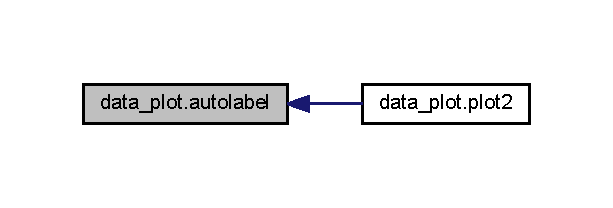
\includegraphics[width=294pt]{namespacedata__plot_ab1e2fbbf96e3102b5af9834fd2a9afe6_icgraph}
\end{center}
\end{figure}


\hypertarget{namespacedata__plot_a561eca3a1a19ba1dd334d4ebabbb62d8}{\index{data\-\_\-plot@{data\-\_\-plot}!get\-\_\-colours@{get\-\_\-colours}}
\index{get\-\_\-colours@{get\-\_\-colours}!data_plot@{data\-\_\-plot}}
\subsubsection[{get\-\_\-colours}]{\setlength{\rightskip}{0pt plus 5cm}def data\-\_\-plot.\-get\-\_\-colours (
\begin{DoxyParamCaption}
\item[{}]{n}
\end{DoxyParamCaption}
)}}\label{namespacedata__plot_a561eca3a1a19ba1dd334d4ebabbb62d8}
\begin{DoxyVerb}Return n pastel colours. \end{DoxyVerb}
 

Here is the call graph for this function\-:
\nopagebreak
\begin{figure}[H]
\begin{center}
\leavevmode
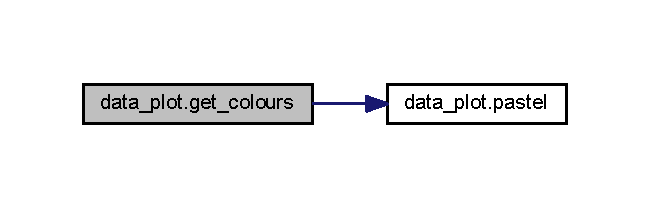
\includegraphics[width=312pt]{namespacedata__plot_a561eca3a1a19ba1dd334d4ebabbb62d8_cgraph}
\end{center}
\end{figure}




Here is the caller graph for this function\-:
\nopagebreak
\begin{figure}[H]
\begin{center}
\leavevmode
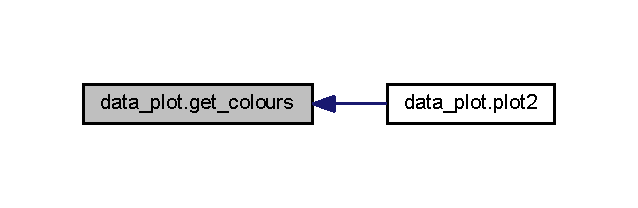
\includegraphics[width=306pt]{namespacedata__plot_a561eca3a1a19ba1dd334d4ebabbb62d8_icgraph}
\end{center}
\end{figure}


\hypertarget{namespacedata__plot_aa83ee5efa7f8257501db891963e6cd42}{\index{data\-\_\-plot@{data\-\_\-plot}!pastel@{pastel}}
\index{pastel@{pastel}!data_plot@{data\-\_\-plot}}
\subsubsection[{pastel}]{\setlength{\rightskip}{0pt plus 5cm}def data\-\_\-plot.\-pastel (
\begin{DoxyParamCaption}
\item[{}]{colour, }
\item[{}]{weight = {\ttfamily 2.4}}
\end{DoxyParamCaption}
)}}\label{namespacedata__plot_aa83ee5efa7f8257501db891963e6cd42}
\begin{DoxyVerb}Convert colour into a nice pastel shade\end{DoxyVerb}
 

Here is the caller graph for this function\-:
\nopagebreak
\begin{figure}[H]
\begin{center}
\leavevmode
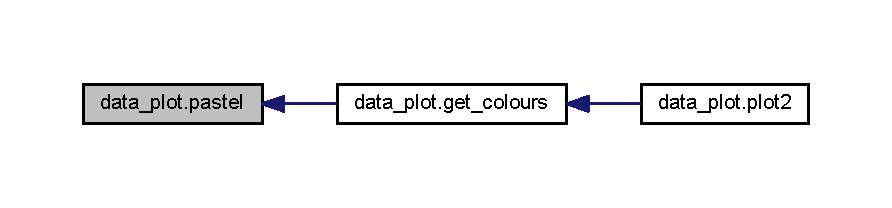
\includegraphics[width=350pt]{namespacedata__plot_aa83ee5efa7f8257501db891963e6cd42_icgraph}
\end{center}
\end{figure}


\hypertarget{namespacedata__plot_ae5595ad2b553b397c5737236e68b5ac0}{\index{data\-\_\-plot@{data\-\_\-plot}!plot2@{plot2}}
\index{plot2@{plot2}!data_plot@{data\-\_\-plot}}
\subsubsection[{plot2}]{\setlength{\rightskip}{0pt plus 5cm}def data\-\_\-plot.\-plot2 (
\begin{DoxyParamCaption}
\item[{}]{dm}
\end{DoxyParamCaption}
)}}\label{namespacedata__plot_ae5595ad2b553b397c5737236e68b5ac0}


Here is the call graph for this function\-:
\nopagebreak
\begin{figure}[H]
\begin{center}
\leavevmode
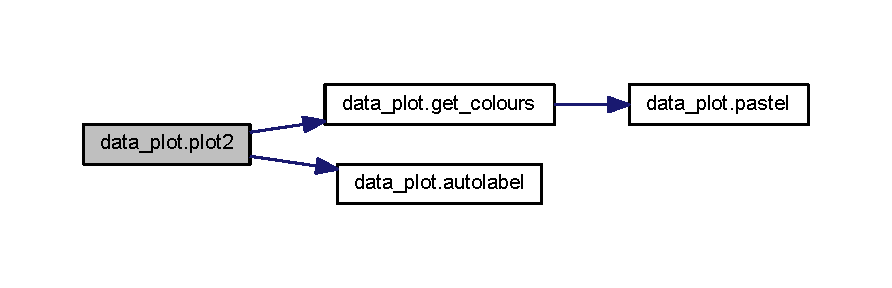
\includegraphics[width=350pt]{namespacedata__plot_ae5595ad2b553b397c5737236e68b5ac0_cgraph}
\end{center}
\end{figure}




\subsection{Variable Documentation}
\hypertarget{namespacedata__plot_a059a797dd0a7e613b2712934dc64140a}{\index{data\-\_\-plot@{data\-\_\-plot}!dm@{dm}}
\index{dm@{dm}!data_plot@{data\-\_\-plot}}
\subsubsection[{dm}]{\setlength{\rightskip}{0pt plus 5cm}tuple data\-\_\-plot.\-dm = pickle.\-load({\bf fload})}}\label{namespacedata__plot_a059a797dd0a7e613b2712934dc64140a}
\hypertarget{namespacedata__plot_ab643ddfd537318e86ad280cd29d6c741}{\index{data\-\_\-plot@{data\-\_\-plot}!fload@{fload}}
\index{fload@{fload}!data_plot@{data\-\_\-plot}}
\subsubsection[{fload}]{\setlength{\rightskip}{0pt plus 5cm}tuple data\-\_\-plot.\-fload = open(sys.\-argv\mbox{[}1\mbox{]}+\char`\"{}.dat\char`\"{},'r')}}\label{namespacedata__plot_ab643ddfd537318e86ad280cd29d6c741}

\hypertarget{namespacedata__struct}{\section{data\-\_\-struct Namespace Reference}
\label{namespacedata__struct}\index{data\-\_\-struct@{data\-\_\-struct}}
}
\subsection*{Classes}
\begin{DoxyCompactItemize}
\item 
class \hyperlink{classdata__struct_1_1_data_struct}{Data\-Struct}
\end{DoxyCompactItemize}

\hypertarget{namespacemodel__template}{\section{model\-\_\-template Namespace Reference}
\label{namespacemodel__template}\index{model\-\_\-template@{model\-\_\-template}}
}
\subsection*{Classes}
\begin{DoxyCompactItemize}
\item 
class \hyperlink{classmodel__template_1_1_model_template}{Model\-Template}
\end{DoxyCompactItemize}

\hypertarget{namespace_models}{\section{Models Namespace Reference}
\label{namespace_models}\index{Models@{Models}}
}
\subsection*{Namespaces}
\begin{DoxyCompactItemize}
\item 
namespace \hyperlink{namespace_models_1_1_g0}{G0}
\item 
namespace \hyperlink{namespace_models_1_1_g0s}{G0s}
\item 
namespace \hyperlink{namespace_models_1_1_g0s_r}{G0s\-R}
\item 
namespace \hyperlink{namespace_models_1_1_g0s_rcon}{G0s\-Rcon}
\item 
namespace \hyperlink{namespace_models_1_1_gqs_r}{Gqs\-R}
\item 
namespace \hyperlink{namespace_models_1_1_gqs_r2}{Gqs\-R2}
\item 
namespace \hyperlink{namespace_models_1_1_gqs_rcon}{Gqs\-Rcon}
\end{DoxyCompactItemize}

\hypertarget{namespace_models_1_1_g0}{\section{Models.\-G0 Namespace Reference}
\label{namespace_models_1_1_g0}\index{Models.\-G0@{Models.\-G0}}
}
\subsection*{Classes}
\begin{DoxyCompactItemize}
\item 
class \hyperlink{class_models_1_1_g0_1_1_model}{Model}
\end{DoxyCompactItemize}

\hypertarget{namespace_models_1_1_g0s}{\section{Models.\-G0s Namespace Reference}
\label{namespace_models_1_1_g0s}\index{Models.\-G0s@{Models.\-G0s}}
}
\subsection*{Classes}
\begin{DoxyCompactItemize}
\item 
class \hyperlink{class_models_1_1_g0s_1_1_model}{Model}
\end{DoxyCompactItemize}

\hypertarget{namespace_models_1_1_g0s_r}{\section{Models.\-G0s\-R Namespace Reference}
\label{namespace_models_1_1_g0s_r}\index{Models.\-G0s\-R@{Models.\-G0s\-R}}
}
\subsection*{Classes}
\begin{DoxyCompactItemize}
\item 
class \hyperlink{class_models_1_1_g0s_r_1_1_model}{Model}
\end{DoxyCompactItemize}

\hypertarget{namespace_models_1_1_g0s_rcon}{\section{Models.\-G0s\-Rcon Namespace Reference}
\label{namespace_models_1_1_g0s_rcon}\index{Models.\-G0s\-Rcon@{Models.\-G0s\-Rcon}}
}
\subsection*{Classes}
\begin{DoxyCompactItemize}
\item 
class \hyperlink{class_models_1_1_g0s_rcon_1_1_model}{Model}
\end{DoxyCompactItemize}

\hypertarget{namespace_models_1_1_gqs_r}{\section{Models.\-Gqs\-R Namespace Reference}
\label{namespace_models_1_1_gqs_r}\index{Models.\-Gqs\-R@{Models.\-Gqs\-R}}
}
\subsection*{Classes}
\begin{DoxyCompactItemize}
\item 
class \hyperlink{class_models_1_1_gqs_r_1_1_model}{Model}
\end{DoxyCompactItemize}

\hypertarget{namespace_models_1_1_gqs_r2}{\section{Models.\-Gqs\-R2 Namespace Reference}
\label{namespace_models_1_1_gqs_r2}\index{Models.\-Gqs\-R2@{Models.\-Gqs\-R2}}
}
\subsection*{Classes}
\begin{DoxyCompactItemize}
\item 
class \hyperlink{class_models_1_1_gqs_r2_1_1_model}{Model}
\end{DoxyCompactItemize}

\hypertarget{namespace_models_1_1_gqs_rcon}{\section{Models.\-Gqs\-Rcon Namespace Reference}
\label{namespace_models_1_1_gqs_rcon}\index{Models.\-Gqs\-Rcon@{Models.\-Gqs\-Rcon}}
}
\subsection*{Classes}
\begin{DoxyCompactItemize}
\item 
class \hyperlink{class_models_1_1_gqs_rcon_1_1_model}{Model}
\end{DoxyCompactItemize}

\hypertarget{namespaceqsim}{\section{qsim Namespace Reference}
\label{namespaceqsim}\index{qsim@{qsim}}
}
\subsection*{Functions}
\begin{DoxyCompactItemize}
\item 
def \hyperlink{namespaceqsim_a96af7f2008e776c37db4a793ee88aa60}{main}
\end{DoxyCompactItemize}


\subsection{Function Documentation}
\hypertarget{namespaceqsim_a96af7f2008e776c37db4a793ee88aa60}{\index{qsim@{qsim}!main@{main}}
\index{main@{main}!qsim@{qsim}}
\subsubsection[{main}]{\setlength{\rightskip}{0pt plus 5cm}def qsim.\-main (
\begin{DoxyParamCaption}
{}
\end{DoxyParamCaption}
)}}\label{namespaceqsim_a96af7f2008e776c37db4a793ee88aa60}

\hypertarget{namespacetest}{\section{test Namespace Reference}
\label{namespacetest}\index{test@{test}}
}
\subsection*{Functions}
\begin{DoxyCompactItemize}
\item 
def \hyperlink{namespacetest_aad79eb47bf4d6f10c684cad8600bca58}{main}
\end{DoxyCompactItemize}


\subsection{Function Documentation}
\hypertarget{namespacetest_aad79eb47bf4d6f10c684cad8600bca58}{\index{test@{test}!main@{main}}
\index{main@{main}!test@{test}}
\subsubsection[{main}]{\setlength{\rightskip}{0pt plus 5cm}def test.\-main (
\begin{DoxyParamCaption}
{}
\end{DoxyParamCaption}
)}}\label{namespacetest_aad79eb47bf4d6f10c684cad8600bca58}

\hypertarget{namespacetest___c_f_r}{\section{test\-\_\-\-C\-F\-R Namespace Reference}
\label{namespacetest___c_f_r}\index{test\-\_\-\-C\-F\-R@{test\-\_\-\-C\-F\-R}}
}
\subsection*{Variables}
\begin{DoxyCompactItemize}
\item 
tuple \hyperlink{namespacetest___c_f_r_a2788cbd1c3e51006f7adc65ba92ac4db}{file\-Stream} = open(\char`\"{}qsim-\/config.\-txt\char`\"{},\char`\"{}r\char`\"{})
\item 
tuple \hyperlink{namespacetest___c_f_r_abc1c0f00adf65dd018a7d9ede57946d0}{curr\-File} = \hyperlink{classcustom__file__reader_1_1_custom_file_reader}{custom\-\_\-file\-\_\-reader.\-Custom\-File\-Reader}(\hyperlink{namespacetest___c_f_r_a2788cbd1c3e51006f7adc65ba92ac4db}{file\-Stream},'horizontal','str')
\item 
tuple \hyperlink{namespacetest___c_f_r_ad4fc1ef0fa68ca6720f5ec10f7e26974}{dd} = curr\-File.\-get\-\_\-dict()
\end{DoxyCompactItemize}


\subsection{Variable Documentation}
\hypertarget{namespacetest___c_f_r_abc1c0f00adf65dd018a7d9ede57946d0}{\index{test\-\_\-\-C\-F\-R@{test\-\_\-\-C\-F\-R}!curr\-File@{curr\-File}}
\index{curr\-File@{curr\-File}!test_CFR@{test\-\_\-\-C\-F\-R}}
\subsubsection[{curr\-File}]{\setlength{\rightskip}{0pt plus 5cm}tuple test\-\_\-\-C\-F\-R.\-curr\-File = {\bf custom\-\_\-file\-\_\-reader.\-Custom\-File\-Reader}({\bf file\-Stream},'horizontal','str')}}\label{namespacetest___c_f_r_abc1c0f00adf65dd018a7d9ede57946d0}
\hypertarget{namespacetest___c_f_r_ad4fc1ef0fa68ca6720f5ec10f7e26974}{\index{test\-\_\-\-C\-F\-R@{test\-\_\-\-C\-F\-R}!dd@{dd}}
\index{dd@{dd}!test_CFR@{test\-\_\-\-C\-F\-R}}
\subsubsection[{dd}]{\setlength{\rightskip}{0pt plus 5cm}tuple test\-\_\-\-C\-F\-R.\-dd = curr\-File.\-get\-\_\-dict()}}\label{namespacetest___c_f_r_ad4fc1ef0fa68ca6720f5ec10f7e26974}
\hypertarget{namespacetest___c_f_r_a2788cbd1c3e51006f7adc65ba92ac4db}{\index{test\-\_\-\-C\-F\-R@{test\-\_\-\-C\-F\-R}!file\-Stream@{file\-Stream}}
\index{file\-Stream@{file\-Stream}!test_CFR@{test\-\_\-\-C\-F\-R}}
\subsubsection[{file\-Stream}]{\setlength{\rightskip}{0pt plus 5cm}tuple test\-\_\-\-C\-F\-R.\-file\-Stream = open(\char`\"{}qsim-\/config.\-txt\char`\"{},\char`\"{}r\char`\"{})}}\label{namespacetest___c_f_r_a2788cbd1c3e51006f7adc65ba92ac4db}

\chapter{Class Documentation}
\hypertarget{classcustom__file__reader_1_1_custom_file_reader}{\section{custom\-\_\-file\-\_\-reader.\-Custom\-File\-Reader Class Reference}
\label{classcustom__file__reader_1_1_custom_file_reader}\index{custom\-\_\-file\-\_\-reader.\-Custom\-File\-Reader@{custom\-\_\-file\-\_\-reader.\-Custom\-File\-Reader}}
}


Inheritance diagram for custom\-\_\-file\-\_\-reader.\-Custom\-File\-Reader\-:
\nopagebreak
\begin{figure}[H]
\begin{center}
\leavevmode
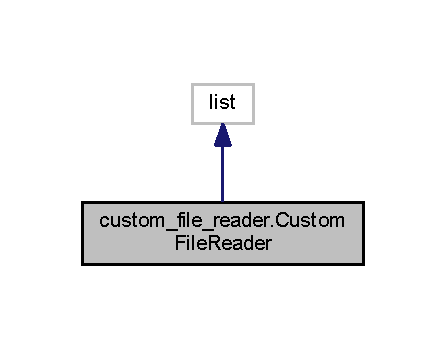
\includegraphics[width=214pt]{classcustom__file__reader_1_1_custom_file_reader__inherit__graph}
\end{center}
\end{figure}


Collaboration diagram for custom\-\_\-file\-\_\-reader.\-Custom\-File\-Reader\-:
\nopagebreak
\begin{figure}[H]
\begin{center}
\leavevmode
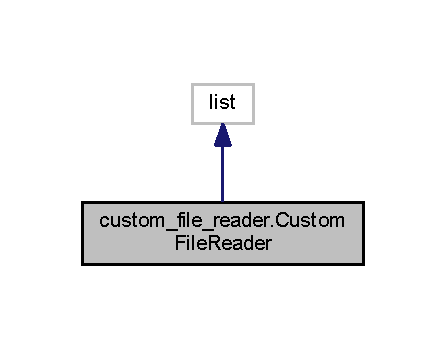
\includegraphics[width=214pt]{classcustom__file__reader_1_1_custom_file_reader__coll__graph}
\end{center}
\end{figure}
\subsection*{Public Member Functions}
\begin{DoxyCompactItemize}
\item 
def \hyperlink{classcustom__file__reader_1_1_custom_file_reader_ae30508851658f07eb975c973678c53a2}{\-\_\-\-\_\-init\-\_\-\-\_\-}
\item 
def \hyperlink{classcustom__file__reader_1_1_custom_file_reader_aa11c4ebcaffc5dd67222fcaccb5e4dab}{read\-\_\-data\-\_\-file}
\item 
def \hyperlink{classcustom__file__reader_1_1_custom_file_reader_a94927010da6c9358cd11cc79e37aa796}{get\-\_\-dict}
\end{DoxyCompactItemize}
\subsection*{Public Attributes}
\begin{DoxyCompactItemize}
\item 
\hyperlink{classcustom__file__reader_1_1_custom_file_reader_a219137e4cd4de13f1159979b3f8e95ea}{parser\-\_\-string}
\item 
\hyperlink{classcustom__file__reader_1_1_custom_file_reader_ab65f0b169e3a73961db6b0501ffb02d0}{type}
\end{DoxyCompactItemize}


\subsection{Detailed Description}
\begin{DoxyVerb}Lector de archivos de texto en diversos formatos personalizados. 

**3 tipos de estructura de archivos: **

- verticales ('vertical'), corresponden a archivos de la forma

label1  label2  label3
x1  y1  z1
x2  y2  z2

-horizontales ('horizontal'): de la forma

label1  x1  x2
label2  y1  y2

-matriciales ('matrix') de la forma

    label1  label2  label3
labela  x1  x2  x3
labelb  x4  x5  x6
labelc  x7  x8  x9

** 3 tipos de parser soportados **
Los datos se leen como strings por defecto. Es posible precisar un parser de los siguientes:

- 'float': lee y almacena los datos como tipo float
- 'int': lee y almacena los datos como tipo int

- 'str': tipo por defecto, lee y almacena los datos como string.

Los labels siempre se leen como string.\end{DoxyVerb}
 

\subsection{Constructor \& Destructor Documentation}
\hypertarget{classcustom__file__reader_1_1_custom_file_reader_ae30508851658f07eb975c973678c53a2}{\index{custom\-\_\-file\-\_\-reader\-::\-Custom\-File\-Reader@{custom\-\_\-file\-\_\-reader\-::\-Custom\-File\-Reader}!\-\_\-\-\_\-init\-\_\-\-\_\-@{\-\_\-\-\_\-init\-\_\-\-\_\-}}
\index{\-\_\-\-\_\-init\-\_\-\-\_\-@{\-\_\-\-\_\-init\-\_\-\-\_\-}!custom_file_reader::CustomFileReader@{custom\-\_\-file\-\_\-reader\-::\-Custom\-File\-Reader}}
\subsubsection[{\-\_\-\-\_\-init\-\_\-\-\_\-}]{\setlength{\rightskip}{0pt plus 5cm}def custom\-\_\-file\-\_\-reader.\-Custom\-File\-Reader.\-\_\-\-\_\-init\-\_\-\-\_\- (
\begin{DoxyParamCaption}
\item[{}]{self, }
\item[{}]{file\-Stream, }
\item[{}]{type, }
\item[{}]{parser\-\_\-string}
\end{DoxyParamCaption}
)}}\label{classcustom__file__reader_1_1_custom_file_reader_ae30508851658f07eb975c973678c53a2}


Here is the call graph for this function\-:
\nopagebreak
\begin{figure}[H]
\begin{center}
\leavevmode
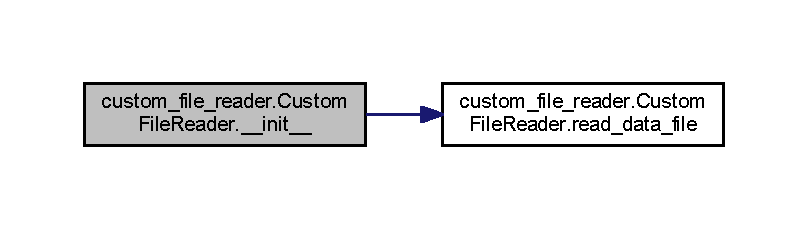
\includegraphics[width=350pt]{classcustom__file__reader_1_1_custom_file_reader_ae30508851658f07eb975c973678c53a2_cgraph}
\end{center}
\end{figure}




\subsection{Member Function Documentation}
\hypertarget{classcustom__file__reader_1_1_custom_file_reader_a94927010da6c9358cd11cc79e37aa796}{\index{custom\-\_\-file\-\_\-reader\-::\-Custom\-File\-Reader@{custom\-\_\-file\-\_\-reader\-::\-Custom\-File\-Reader}!get\-\_\-dict@{get\-\_\-dict}}
\index{get\-\_\-dict@{get\-\_\-dict}!custom_file_reader::CustomFileReader@{custom\-\_\-file\-\_\-reader\-::\-Custom\-File\-Reader}}
\subsubsection[{get\-\_\-dict}]{\setlength{\rightskip}{0pt plus 5cm}def custom\-\_\-file\-\_\-reader.\-Custom\-File\-Reader.\-get\-\_\-dict (
\begin{DoxyParamCaption}
\item[{}]{self}
\end{DoxyParamCaption}
)}}\label{classcustom__file__reader_1_1_custom_file_reader_a94927010da6c9358cd11cc79e37aa796}
\hypertarget{classcustom__file__reader_1_1_custom_file_reader_aa11c4ebcaffc5dd67222fcaccb5e4dab}{\index{custom\-\_\-file\-\_\-reader\-::\-Custom\-File\-Reader@{custom\-\_\-file\-\_\-reader\-::\-Custom\-File\-Reader}!read\-\_\-data\-\_\-file@{read\-\_\-data\-\_\-file}}
\index{read\-\_\-data\-\_\-file@{read\-\_\-data\-\_\-file}!custom_file_reader::CustomFileReader@{custom\-\_\-file\-\_\-reader\-::\-Custom\-File\-Reader}}
\subsubsection[{read\-\_\-data\-\_\-file}]{\setlength{\rightskip}{0pt plus 5cm}def custom\-\_\-file\-\_\-reader.\-Custom\-File\-Reader.\-read\-\_\-data\-\_\-file (
\begin{DoxyParamCaption}
\item[{}]{self}
\end{DoxyParamCaption}
)}}\label{classcustom__file__reader_1_1_custom_file_reader_aa11c4ebcaffc5dd67222fcaccb5e4dab}


Here is the caller graph for this function\-:
\nopagebreak
\begin{figure}[H]
\begin{center}
\leavevmode
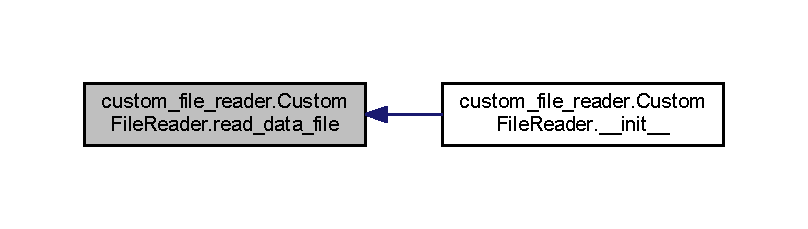
\includegraphics[width=350pt]{classcustom__file__reader_1_1_custom_file_reader_aa11c4ebcaffc5dd67222fcaccb5e4dab_icgraph}
\end{center}
\end{figure}




\subsection{Member Data Documentation}
\hypertarget{classcustom__file__reader_1_1_custom_file_reader_a219137e4cd4de13f1159979b3f8e95ea}{\index{custom\-\_\-file\-\_\-reader\-::\-Custom\-File\-Reader@{custom\-\_\-file\-\_\-reader\-::\-Custom\-File\-Reader}!parser\-\_\-string@{parser\-\_\-string}}
\index{parser\-\_\-string@{parser\-\_\-string}!custom_file_reader::CustomFileReader@{custom\-\_\-file\-\_\-reader\-::\-Custom\-File\-Reader}}
\subsubsection[{parser\-\_\-string}]{\setlength{\rightskip}{0pt plus 5cm}custom\-\_\-file\-\_\-reader.\-Custom\-File\-Reader.\-parser\-\_\-string}}\label{classcustom__file__reader_1_1_custom_file_reader_a219137e4cd4de13f1159979b3f8e95ea}
\hypertarget{classcustom__file__reader_1_1_custom_file_reader_ab65f0b169e3a73961db6b0501ffb02d0}{\index{custom\-\_\-file\-\_\-reader\-::\-Custom\-File\-Reader@{custom\-\_\-file\-\_\-reader\-::\-Custom\-File\-Reader}!type@{type}}
\index{type@{type}!custom_file_reader::CustomFileReader@{custom\-\_\-file\-\_\-reader\-::\-Custom\-File\-Reader}}
\subsubsection[{type}]{\setlength{\rightskip}{0pt plus 5cm}custom\-\_\-file\-\_\-reader.\-Custom\-File\-Reader.\-type}}\label{classcustom__file__reader_1_1_custom_file_reader_ab65f0b169e3a73961db6b0501ffb02d0}


The documentation for this class was generated from the following file\-:\begin{DoxyCompactItemize}
\item 
\hyperlink{custom__file__reader_8py}{custom\-\_\-file\-\_\-reader.\-py}\end{DoxyCompactItemize}

\hypertarget{classdata__manager_1_1_data_manager}{\section{data\-\_\-manager.\-Data\-Manager Class Reference}
\label{classdata__manager_1_1_data_manager}\index{data\-\_\-manager.\-Data\-Manager@{data\-\_\-manager.\-Data\-Manager}}
}


Inheritance diagram for data\-\_\-manager.\-Data\-Manager\-:
\nopagebreak
\begin{figure}[H]
\begin{center}
\leavevmode
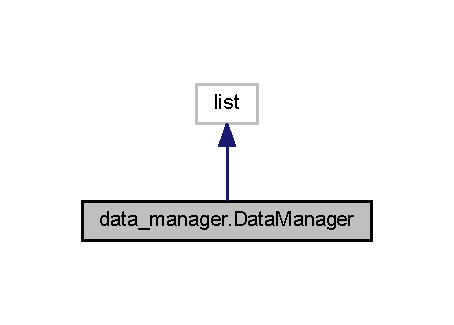
\includegraphics[width=218pt]{classdata__manager_1_1_data_manager__inherit__graph}
\end{center}
\end{figure}


Collaboration diagram for data\-\_\-manager.\-Data\-Manager\-:
\nopagebreak
\begin{figure}[H]
\begin{center}
\leavevmode
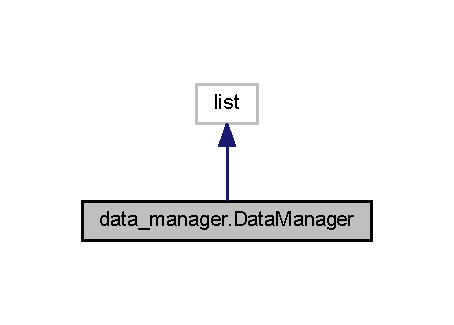
\includegraphics[width=218pt]{classdata__manager_1_1_data_manager__coll__graph}
\end{center}
\end{figure}
\subsection*{Public Member Functions}
\begin{DoxyCompactItemize}
\item 
def \hyperlink{classdata__manager_1_1_data_manager_ac366e9ff1e60bbd9f1af6f03c16786be}{\-\_\-\-\_\-init\-\_\-\-\_\-}
\item 
def \hyperlink{classdata__manager_1_1_data_manager_a1ea4ae2852d3babf339d6b7b9b76ed4e}{unload\-\_\-data\-\_\-from\-\_\-files\-\_\-to\-\_\-dict}
\item 
def \hyperlink{classdata__manager_1_1_data_manager_a129a0af6efb1287dc5300f197091d238}{unload\-\_\-data\-\_\-from\-\_\-dict\-\_\-to\-\_\-vars}
\item 
def \hyperlink{classdata__manager_1_1_data_manager_aa60e6ad57d28146b4c7a5cdba7995313}{init\-\_\-\-H\-\_\-h}
\item 
def \hyperlink{classdata__manager_1_1_data_manager_a8052ab1fb1001bddc131a2fc890e2d0b}{init\-\_\-\-S\-\_\-vi}
\item 
def \hyperlink{classdata__manager_1_1_data_manager_a7b7b6b3233454cbf4ca1a23473d44bbd}{print\-\_\-logfiles}
\item 
def \hyperlink{classdata__manager_1_1_data_manager_ab88775ec4445d6271b5ae56083a18da5}{string\-\_\-output\-\_\-var}
\item 
def \hyperlink{classdata__manager_1_1_data_manager_aeb0578e88299929a3d7496be296cb63d}{time\-\_\-serie\-\_\-var}
\end{DoxyCompactItemize}
\subsection*{Public Attributes}
\begin{DoxyCompactItemize}
\item 
\hyperlink{classdata__manager_1_1_data_manager_ab9b39124c635d1e7babbb3459288d9d3}{N\-O\-M\-B\-R\-E\-\_\-\-D\-A\-T\-A}
\item 
\hyperlink{classdata__manager_1_1_data_manager_accbcc3f4e324250aa60e83d2b155b6ea}{dd}
\item 
\hyperlink{classdata__manager_1_1_data_manager_a4a37984bcecfc9866ee8f16a0c205d6e}{N\-\_\-h}
\item 
\hyperlink{classdata__manager_1_1_data_manager_addad06bf8294cb9e247cfb336402cd5e}{N\-\_\-vi}
\end{DoxyCompactItemize}


\subsection{Detailed Description}
\begin{DoxyVerb}Clase que contiene la data para los modelos\end{DoxyVerb}
 

\subsection{Constructor \& Destructor Documentation}
\hypertarget{classdata__manager_1_1_data_manager_ac366e9ff1e60bbd9f1af6f03c16786be}{\index{data\-\_\-manager\-::\-Data\-Manager@{data\-\_\-manager\-::\-Data\-Manager}!\-\_\-\-\_\-init\-\_\-\-\_\-@{\-\_\-\-\_\-init\-\_\-\-\_\-}}
\index{\-\_\-\-\_\-init\-\_\-\-\_\-@{\-\_\-\-\_\-init\-\_\-\-\_\-}!data_manager::DataManager@{data\-\_\-manager\-::\-Data\-Manager}}
\subsubsection[{\-\_\-\-\_\-init\-\_\-\-\_\-}]{\setlength{\rightskip}{0pt plus 5cm}def data\-\_\-manager.\-Data\-Manager.\-\_\-\-\_\-init\-\_\-\-\_\- (
\begin{DoxyParamCaption}
\item[{}]{self, }
\item[{}]{data\-Folder\-Path, }
\item[{}]{data\-Arg}
\end{DoxyParamCaption}
)}}\label{classdata__manager_1_1_data_manager_ac366e9ff1e60bbd9f1af6f03c16786be}


\subsection{Member Function Documentation}
\hypertarget{classdata__manager_1_1_data_manager_aa60e6ad57d28146b4c7a5cdba7995313}{\index{data\-\_\-manager\-::\-Data\-Manager@{data\-\_\-manager\-::\-Data\-Manager}!init\-\_\-\-H\-\_\-h@{init\-\_\-\-H\-\_\-h}}
\index{init\-\_\-\-H\-\_\-h@{init\-\_\-\-H\-\_\-h}!data_manager::DataManager@{data\-\_\-manager\-::\-Data\-Manager}}
\subsubsection[{init\-\_\-\-H\-\_\-h}]{\setlength{\rightskip}{0pt plus 5cm}def data\-\_\-manager.\-Data\-Manager.\-init\-\_\-\-H\-\_\-h (
\begin{DoxyParamCaption}
\item[{}]{self}
\end{DoxyParamCaption}
)}}\label{classdata__manager_1_1_data_manager_aa60e6ad57d28146b4c7a5cdba7995313}
\hypertarget{classdata__manager_1_1_data_manager_a8052ab1fb1001bddc131a2fc890e2d0b}{\index{data\-\_\-manager\-::\-Data\-Manager@{data\-\_\-manager\-::\-Data\-Manager}!init\-\_\-\-S\-\_\-vi@{init\-\_\-\-S\-\_\-vi}}
\index{init\-\_\-\-S\-\_\-vi@{init\-\_\-\-S\-\_\-vi}!data_manager::DataManager@{data\-\_\-manager\-::\-Data\-Manager}}
\subsubsection[{init\-\_\-\-S\-\_\-vi}]{\setlength{\rightskip}{0pt plus 5cm}def data\-\_\-manager.\-Data\-Manager.\-init\-\_\-\-S\-\_\-vi (
\begin{DoxyParamCaption}
\item[{}]{self}
\end{DoxyParamCaption}
)}}\label{classdata__manager_1_1_data_manager_a8052ab1fb1001bddc131a2fc890e2d0b}
\hypertarget{classdata__manager_1_1_data_manager_a7b7b6b3233454cbf4ca1a23473d44bbd}{\index{data\-\_\-manager\-::\-Data\-Manager@{data\-\_\-manager\-::\-Data\-Manager}!print\-\_\-logfiles@{print\-\_\-logfiles}}
\index{print\-\_\-logfiles@{print\-\_\-logfiles}!data_manager::DataManager@{data\-\_\-manager\-::\-Data\-Manager}}
\subsubsection[{print\-\_\-logfiles}]{\setlength{\rightskip}{0pt plus 5cm}def data\-\_\-manager.\-Data\-Manager.\-print\-\_\-logfiles (
\begin{DoxyParamCaption}
\item[{}]{self, }
\item[{}]{curr\-Output\-Folder\-Path = {\ttfamily \char`\"{}\char`\"{}}}
\end{DoxyParamCaption}
)}}\label{classdata__manager_1_1_data_manager_a7b7b6b3233454cbf4ca1a23473d44bbd}


Here is the call graph for this function\-:
\nopagebreak
\begin{figure}[H]
\begin{center}
\leavevmode
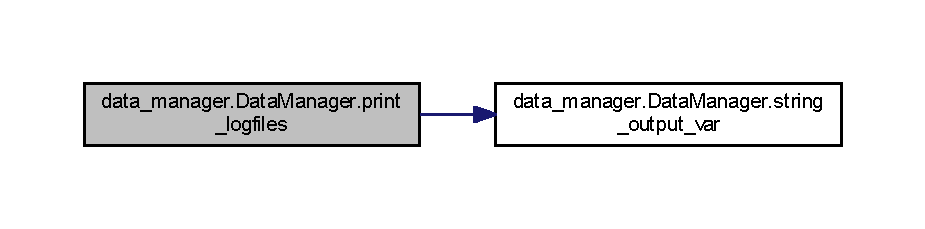
\includegraphics[width=350pt]{classdata__manager_1_1_data_manager_a7b7b6b3233454cbf4ca1a23473d44bbd_cgraph}
\end{center}
\end{figure}


\hypertarget{classdata__manager_1_1_data_manager_ab88775ec4445d6271b5ae56083a18da5}{\index{data\-\_\-manager\-::\-Data\-Manager@{data\-\_\-manager\-::\-Data\-Manager}!string\-\_\-output\-\_\-var@{string\-\_\-output\-\_\-var}}
\index{string\-\_\-output\-\_\-var@{string\-\_\-output\-\_\-var}!data_manager::DataManager@{data\-\_\-manager\-::\-Data\-Manager}}
\subsubsection[{string\-\_\-output\-\_\-var}]{\setlength{\rightskip}{0pt plus 5cm}def data\-\_\-manager.\-Data\-Manager.\-string\-\_\-output\-\_\-var (
\begin{DoxyParamCaption}
\item[{}]{self, }
\item[{}]{var\-Name}
\end{DoxyParamCaption}
)}}\label{classdata__manager_1_1_data_manager_ab88775ec4445d6271b5ae56083a18da5}


Here is the caller graph for this function\-:
\nopagebreak
\begin{figure}[H]
\begin{center}
\leavevmode
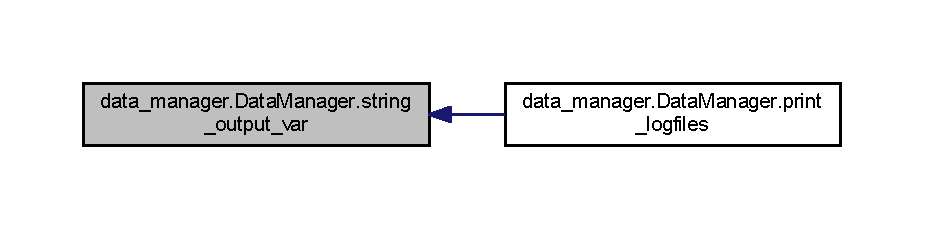
\includegraphics[width=350pt]{classdata__manager_1_1_data_manager_ab88775ec4445d6271b5ae56083a18da5_icgraph}
\end{center}
\end{figure}


\hypertarget{classdata__manager_1_1_data_manager_aeb0578e88299929a3d7496be296cb63d}{\index{data\-\_\-manager\-::\-Data\-Manager@{data\-\_\-manager\-::\-Data\-Manager}!time\-\_\-serie\-\_\-var@{time\-\_\-serie\-\_\-var}}
\index{time\-\_\-serie\-\_\-var@{time\-\_\-serie\-\_\-var}!data_manager::DataManager@{data\-\_\-manager\-::\-Data\-Manager}}
\subsubsection[{time\-\_\-serie\-\_\-var}]{\setlength{\rightskip}{0pt plus 5cm}def data\-\_\-manager.\-Data\-Manager.\-time\-\_\-serie\-\_\-var (
\begin{DoxyParamCaption}
\item[{}]{self, }
\item[{}]{var\-Name}
\end{DoxyParamCaption}
)}}\label{classdata__manager_1_1_data_manager_aeb0578e88299929a3d7496be296cb63d}
\hypertarget{classdata__manager_1_1_data_manager_a129a0af6efb1287dc5300f197091d238}{\index{data\-\_\-manager\-::\-Data\-Manager@{data\-\_\-manager\-::\-Data\-Manager}!unload\-\_\-data\-\_\-from\-\_\-dict\-\_\-to\-\_\-vars@{unload\-\_\-data\-\_\-from\-\_\-dict\-\_\-to\-\_\-vars}}
\index{unload\-\_\-data\-\_\-from\-\_\-dict\-\_\-to\-\_\-vars@{unload\-\_\-data\-\_\-from\-\_\-dict\-\_\-to\-\_\-vars}!data_manager::DataManager@{data\-\_\-manager\-::\-Data\-Manager}}
\subsubsection[{unload\-\_\-data\-\_\-from\-\_\-dict\-\_\-to\-\_\-vars}]{\setlength{\rightskip}{0pt plus 5cm}def data\-\_\-manager.\-Data\-Manager.\-unload\-\_\-data\-\_\-from\-\_\-dict\-\_\-to\-\_\-vars (
\begin{DoxyParamCaption}
\item[{}]{self, }
\item[{}]{dd}
\end{DoxyParamCaption}
)}}\label{classdata__manager_1_1_data_manager_a129a0af6efb1287dc5300f197091d238}
\hypertarget{classdata__manager_1_1_data_manager_a1ea4ae2852d3babf339d6b7b9b76ed4e}{\index{data\-\_\-manager\-::\-Data\-Manager@{data\-\_\-manager\-::\-Data\-Manager}!unload\-\_\-data\-\_\-from\-\_\-files\-\_\-to\-\_\-dict@{unload\-\_\-data\-\_\-from\-\_\-files\-\_\-to\-\_\-dict}}
\index{unload\-\_\-data\-\_\-from\-\_\-files\-\_\-to\-\_\-dict@{unload\-\_\-data\-\_\-from\-\_\-files\-\_\-to\-\_\-dict}!data_manager::DataManager@{data\-\_\-manager\-::\-Data\-Manager}}
\subsubsection[{unload\-\_\-data\-\_\-from\-\_\-files\-\_\-to\-\_\-dict}]{\setlength{\rightskip}{0pt plus 5cm}def data\-\_\-manager.\-Data\-Manager.\-unload\-\_\-data\-\_\-from\-\_\-files\-\_\-to\-\_\-dict (
\begin{DoxyParamCaption}
\item[{}]{self, }
\item[{}]{file\-List}
\end{DoxyParamCaption}
)}}\label{classdata__manager_1_1_data_manager_a1ea4ae2852d3babf339d6b7b9b76ed4e}


\subsection{Member Data Documentation}
\hypertarget{classdata__manager_1_1_data_manager_accbcc3f4e324250aa60e83d2b155b6ea}{\index{data\-\_\-manager\-::\-Data\-Manager@{data\-\_\-manager\-::\-Data\-Manager}!dd@{dd}}
\index{dd@{dd}!data_manager::DataManager@{data\-\_\-manager\-::\-Data\-Manager}}
\subsubsection[{dd}]{\setlength{\rightskip}{0pt plus 5cm}data\-\_\-manager.\-Data\-Manager.\-dd}}\label{classdata__manager_1_1_data_manager_accbcc3f4e324250aa60e83d2b155b6ea}
\hypertarget{classdata__manager_1_1_data_manager_a4a37984bcecfc9866ee8f16a0c205d6e}{\index{data\-\_\-manager\-::\-Data\-Manager@{data\-\_\-manager\-::\-Data\-Manager}!N\-\_\-h@{N\-\_\-h}}
\index{N\-\_\-h@{N\-\_\-h}!data_manager::DataManager@{data\-\_\-manager\-::\-Data\-Manager}}
\subsubsection[{N\-\_\-h}]{\setlength{\rightskip}{0pt plus 5cm}data\-\_\-manager.\-Data\-Manager.\-N\-\_\-h}}\label{classdata__manager_1_1_data_manager_a4a37984bcecfc9866ee8f16a0c205d6e}
\hypertarget{classdata__manager_1_1_data_manager_addad06bf8294cb9e247cfb336402cd5e}{\index{data\-\_\-manager\-::\-Data\-Manager@{data\-\_\-manager\-::\-Data\-Manager}!N\-\_\-vi@{N\-\_\-vi}}
\index{N\-\_\-vi@{N\-\_\-vi}!data_manager::DataManager@{data\-\_\-manager\-::\-Data\-Manager}}
\subsubsection[{N\-\_\-vi}]{\setlength{\rightskip}{0pt plus 5cm}data\-\_\-manager.\-Data\-Manager.\-N\-\_\-vi}}\label{classdata__manager_1_1_data_manager_addad06bf8294cb9e247cfb336402cd5e}
\hypertarget{classdata__manager_1_1_data_manager_ab9b39124c635d1e7babbb3459288d9d3}{\index{data\-\_\-manager\-::\-Data\-Manager@{data\-\_\-manager\-::\-Data\-Manager}!N\-O\-M\-B\-R\-E\-\_\-\-D\-A\-T\-A@{N\-O\-M\-B\-R\-E\-\_\-\-D\-A\-T\-A}}
\index{N\-O\-M\-B\-R\-E\-\_\-\-D\-A\-T\-A@{N\-O\-M\-B\-R\-E\-\_\-\-D\-A\-T\-A}!data_manager::DataManager@{data\-\_\-manager\-::\-Data\-Manager}}
\subsubsection[{N\-O\-M\-B\-R\-E\-\_\-\-D\-A\-T\-A}]{\setlength{\rightskip}{0pt plus 5cm}data\-\_\-manager.\-Data\-Manager.\-N\-O\-M\-B\-R\-E\-\_\-\-D\-A\-T\-A}}\label{classdata__manager_1_1_data_manager_ab9b39124c635d1e7babbb3459288d9d3}


The documentation for this class was generated from the following file\-:\begin{DoxyCompactItemize}
\item 
\hyperlink{data__manager_8py}{data\-\_\-manager.\-py}\end{DoxyCompactItemize}

\hypertarget{classdata__struct_1_1_data_struct}{\section{data\-\_\-struct.\-Data\-Struct Class Reference}
\label{classdata__struct_1_1_data_struct}\index{data\-\_\-struct.\-Data\-Struct@{data\-\_\-struct.\-Data\-Struct}}
}
\subsection*{Public Member Functions}
\begin{DoxyCompactItemize}
\item 
def \hyperlink{classdata__struct_1_1_data_struct_a4446eab90aa49a2cc81f55eb8e8a91a1}{\-\_\-\-\_\-init\-\_\-\-\_\-}
\item 
def \hyperlink{classdata__struct_1_1_data_struct_a29f1a412e9b3f1d72c4620dd5f2469fe}{copy}
\end{DoxyCompactItemize}
\subsection*{Public Attributes}
\begin{DoxyCompactItemize}
\item 
\hyperlink{classdata__struct_1_1_data_struct_ac40cb72bf1a7abf1c62002ac98333697}{var\-\_\-dict}
\end{DoxyCompactItemize}


\subsection{Detailed Description}
\begin{DoxyVerb}Clase que maneja las variables del modelo\end{DoxyVerb}
 

\subsection{Constructor \& Destructor Documentation}
\hypertarget{classdata__struct_1_1_data_struct_a4446eab90aa49a2cc81f55eb8e8a91a1}{\index{data\-\_\-struct\-::\-Data\-Struct@{data\-\_\-struct\-::\-Data\-Struct}!\-\_\-\-\_\-init\-\_\-\-\_\-@{\-\_\-\-\_\-init\-\_\-\-\_\-}}
\index{\-\_\-\-\_\-init\-\_\-\-\_\-@{\-\_\-\-\_\-init\-\_\-\-\_\-}!data_struct::DataStruct@{data\-\_\-struct\-::\-Data\-Struct}}
\subsubsection[{\-\_\-\-\_\-init\-\_\-\-\_\-}]{\setlength{\rightskip}{0pt plus 5cm}def data\-\_\-struct.\-Data\-Struct.\-\_\-\-\_\-init\-\_\-\-\_\- (
\begin{DoxyParamCaption}
\item[{}]{self, }
\item[{}]{N\-\_\-h, }
\item[{}]{N\-\_\-vi}
\end{DoxyParamCaption}
)}}\label{classdata__struct_1_1_data_struct_a4446eab90aa49a2cc81f55eb8e8a91a1}


\subsection{Member Function Documentation}
\hypertarget{classdata__struct_1_1_data_struct_a29f1a412e9b3f1d72c4620dd5f2469fe}{\index{data\-\_\-struct\-::\-Data\-Struct@{data\-\_\-struct\-::\-Data\-Struct}!copy@{copy}}
\index{copy@{copy}!data_struct::DataStruct@{data\-\_\-struct\-::\-Data\-Struct}}
\subsubsection[{copy}]{\setlength{\rightskip}{0pt plus 5cm}def data\-\_\-struct.\-Data\-Struct.\-copy (
\begin{DoxyParamCaption}
\item[{}]{self}
\end{DoxyParamCaption}
)}}\label{classdata__struct_1_1_data_struct_a29f1a412e9b3f1d72c4620dd5f2469fe}


\subsection{Member Data Documentation}
\hypertarget{classdata__struct_1_1_data_struct_ac40cb72bf1a7abf1c62002ac98333697}{\index{data\-\_\-struct\-::\-Data\-Struct@{data\-\_\-struct\-::\-Data\-Struct}!var\-\_\-dict@{var\-\_\-dict}}
\index{var\-\_\-dict@{var\-\_\-dict}!data_struct::DataStruct@{data\-\_\-struct\-::\-Data\-Struct}}
\subsubsection[{var\-\_\-dict}]{\setlength{\rightskip}{0pt plus 5cm}data\-\_\-struct.\-Data\-Struct.\-var\-\_\-dict}}\label{classdata__struct_1_1_data_struct_ac40cb72bf1a7abf1c62002ac98333697}


The documentation for this class was generated from the following file\-:\begin{DoxyCompactItemize}
\item 
\hyperlink{data__struct_8py}{data\-\_\-struct.\-py}\end{DoxyCompactItemize}

\hypertarget{class_models_1_1_gqs_r2_1_1_model}{\section{Models.\-Gqs\-R2.\-Model Class Reference}
\label{class_models_1_1_gqs_r2_1_1_model}\index{Models.\-Gqs\-R2.\-Model@{Models.\-Gqs\-R2.\-Model}}
}


Inheritance diagram for Models.\-Gqs\-R2.\-Model\-:
\nopagebreak
\begin{figure}[H]
\begin{center}
\leavevmode
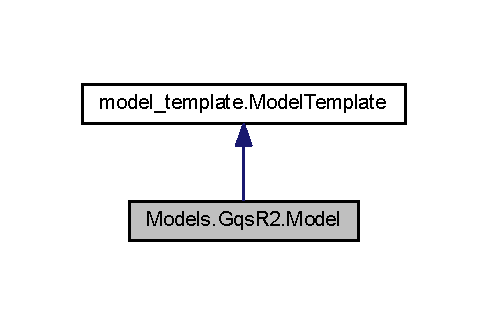
\includegraphics[width=234pt]{class_models_1_1_gqs_r2_1_1_model__inherit__graph}
\end{center}
\end{figure}


Collaboration diagram for Models.\-Gqs\-R2.\-Model\-:
\nopagebreak
\begin{figure}[H]
\begin{center}
\leavevmode
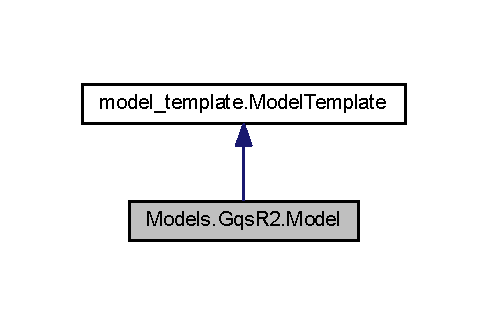
\includegraphics[width=234pt]{class_models_1_1_gqs_r2_1_1_model__coll__graph}
\end{center}
\end{figure}
\subsection*{Public Member Functions}
\begin{DoxyCompactItemize}
\item 
def \hyperlink{class_models_1_1_gqs_r2_1_1_model_ab2cd98d7a4a1218895cba074772cc4c4}{\-\_\-\-\_\-init\-\_\-\-\_\-}
\item 
def \hyperlink{class_models_1_1_gqs_r2_1_1_model_a23cf151ce884bc5190aaedd9213370ad}{calc\-\_\-b\-\_\-h\-\_\-vi}
\item 
def \hyperlink{class_models_1_1_gqs_r2_1_1_model_a46b271129aa9f472f601c7913fdb8552}{calc\-\_\-b\-\_\-h}
\item 
def \hyperlink{class_models_1_1_gqs_r2_1_1_model_a2844fd5f69ed998c4107f9e640e658c2}{calc\-\_\-\-P\-\_\-h\-\_\-vi}
\item 
def \hyperlink{class_models_1_1_gqs_r2_1_1_model_ad8990b8b34c861fc0dfe45f522e8e9b5}{calc\-\_\-r\-\_\-vi}
\item 
def \hyperlink{class_models_1_1_gqs_r2_1_1_model_a03e0134c6b3dc566f470bf65f62822e7}{calc\-\_\-\-S\-\_\-vi}
\item 
def \hyperlink{class_models_1_1_gqs_r2_1_1_model_a2fd6b30a63cb9b97b69f9ee61ffe747d}{calc\-\_\-gamma\-\_\-vi}
\end{DoxyCompactItemize}
\subsection*{Additional Inherited Members}


\subsection{Detailed Description}
\begin{DoxyVerb}Modelo\end{DoxyVerb}
 

\subsection{Constructor \& Destructor Documentation}
\hypertarget{class_models_1_1_gqs_r2_1_1_model_ab2cd98d7a4a1218895cba074772cc4c4}{\index{Models\-::\-Gqs\-R2\-::\-Model@{Models\-::\-Gqs\-R2\-::\-Model}!\-\_\-\-\_\-init\-\_\-\-\_\-@{\-\_\-\-\_\-init\-\_\-\-\_\-}}
\index{\-\_\-\-\_\-init\-\_\-\-\_\-@{\-\_\-\-\_\-init\-\_\-\-\_\-}!Models::GqsR2::Model@{Models\-::\-Gqs\-R2\-::\-Model}}
\subsubsection[{\-\_\-\-\_\-init\-\_\-\-\_\-}]{\setlength{\rightskip}{0pt plus 5cm}def Models.\-Gqs\-R2.\-Model.\-\_\-\-\_\-init\-\_\-\-\_\- (
\begin{DoxyParamCaption}
\item[{}]{self, }
\item[{}]{model\-Name}
\end{DoxyParamCaption}
)}}\label{class_models_1_1_gqs_r2_1_1_model_ab2cd98d7a4a1218895cba074772cc4c4}


\subsection{Member Function Documentation}
\hypertarget{class_models_1_1_gqs_r2_1_1_model_a46b271129aa9f472f601c7913fdb8552}{\index{Models\-::\-Gqs\-R2\-::\-Model@{Models\-::\-Gqs\-R2\-::\-Model}!calc\-\_\-b\-\_\-h@{calc\-\_\-b\-\_\-h}}
\index{calc\-\_\-b\-\_\-h@{calc\-\_\-b\-\_\-h}!Models::GqsR2::Model@{Models\-::\-Gqs\-R2\-::\-Model}}
\subsubsection[{calc\-\_\-b\-\_\-h}]{\setlength{\rightskip}{0pt plus 5cm}def Models.\-Gqs\-R2.\-Model.\-calc\-\_\-b\-\_\-h (
\begin{DoxyParamCaption}
\item[{}]{self, }
\item[{}]{dm, }
\item[{}]{t}
\end{DoxyParamCaption}
)}}\label{class_models_1_1_gqs_r2_1_1_model_a46b271129aa9f472f601c7913fdb8552}
\hypertarget{class_models_1_1_gqs_r2_1_1_model_a23cf151ce884bc5190aaedd9213370ad}{\index{Models\-::\-Gqs\-R2\-::\-Model@{Models\-::\-Gqs\-R2\-::\-Model}!calc\-\_\-b\-\_\-h\-\_\-vi@{calc\-\_\-b\-\_\-h\-\_\-vi}}
\index{calc\-\_\-b\-\_\-h\-\_\-vi@{calc\-\_\-b\-\_\-h\-\_\-vi}!Models::GqsR2::Model@{Models\-::\-Gqs\-R2\-::\-Model}}
\subsubsection[{calc\-\_\-b\-\_\-h\-\_\-vi}]{\setlength{\rightskip}{0pt plus 5cm}def Models.\-Gqs\-R2.\-Model.\-calc\-\_\-b\-\_\-h\-\_\-vi (
\begin{DoxyParamCaption}
\item[{}]{self, }
\item[{}]{dm, }
\item[{}]{t}
\end{DoxyParamCaption}
)}}\label{class_models_1_1_gqs_r2_1_1_model_a23cf151ce884bc5190aaedd9213370ad}
\hypertarget{class_models_1_1_gqs_r2_1_1_model_a2fd6b30a63cb9b97b69f9ee61ffe747d}{\index{Models\-::\-Gqs\-R2\-::\-Model@{Models\-::\-Gqs\-R2\-::\-Model}!calc\-\_\-gamma\-\_\-vi@{calc\-\_\-gamma\-\_\-vi}}
\index{calc\-\_\-gamma\-\_\-vi@{calc\-\_\-gamma\-\_\-vi}!Models::GqsR2::Model@{Models\-::\-Gqs\-R2\-::\-Model}}
\subsubsection[{calc\-\_\-gamma\-\_\-vi}]{\setlength{\rightskip}{0pt plus 5cm}def Models.\-Gqs\-R2.\-Model.\-calc\-\_\-gamma\-\_\-vi (
\begin{DoxyParamCaption}
\item[{}]{self, }
\item[{}]{dm, }
\item[{}]{t}
\end{DoxyParamCaption}
)}}\label{class_models_1_1_gqs_r2_1_1_model_a2fd6b30a63cb9b97b69f9ee61ffe747d}
\hypertarget{class_models_1_1_gqs_r2_1_1_model_a2844fd5f69ed998c4107f9e640e658c2}{\index{Models\-::\-Gqs\-R2\-::\-Model@{Models\-::\-Gqs\-R2\-::\-Model}!calc\-\_\-\-P\-\_\-h\-\_\-vi@{calc\-\_\-\-P\-\_\-h\-\_\-vi}}
\index{calc\-\_\-\-P\-\_\-h\-\_\-vi@{calc\-\_\-\-P\-\_\-h\-\_\-vi}!Models::GqsR2::Model@{Models\-::\-Gqs\-R2\-::\-Model}}
\subsubsection[{calc\-\_\-\-P\-\_\-h\-\_\-vi}]{\setlength{\rightskip}{0pt plus 5cm}def Models.\-Gqs\-R2.\-Model.\-calc\-\_\-\-P\-\_\-h\-\_\-vi (
\begin{DoxyParamCaption}
\item[{}]{self, }
\item[{}]{dm, }
\item[{}]{t}
\end{DoxyParamCaption}
)}}\label{class_models_1_1_gqs_r2_1_1_model_a2844fd5f69ed998c4107f9e640e658c2}
\hypertarget{class_models_1_1_gqs_r2_1_1_model_ad8990b8b34c861fc0dfe45f522e8e9b5}{\index{Models\-::\-Gqs\-R2\-::\-Model@{Models\-::\-Gqs\-R2\-::\-Model}!calc\-\_\-r\-\_\-vi@{calc\-\_\-r\-\_\-vi}}
\index{calc\-\_\-r\-\_\-vi@{calc\-\_\-r\-\_\-vi}!Models::GqsR2::Model@{Models\-::\-Gqs\-R2\-::\-Model}}
\subsubsection[{calc\-\_\-r\-\_\-vi}]{\setlength{\rightskip}{0pt plus 5cm}def Models.\-Gqs\-R2.\-Model.\-calc\-\_\-r\-\_\-vi (
\begin{DoxyParamCaption}
\item[{}]{self, }
\item[{}]{dm, }
\item[{}]{t}
\end{DoxyParamCaption}
)}}\label{class_models_1_1_gqs_r2_1_1_model_ad8990b8b34c861fc0dfe45f522e8e9b5}
\hypertarget{class_models_1_1_gqs_r2_1_1_model_a03e0134c6b3dc566f470bf65f62822e7}{\index{Models\-::\-Gqs\-R2\-::\-Model@{Models\-::\-Gqs\-R2\-::\-Model}!calc\-\_\-\-S\-\_\-vi@{calc\-\_\-\-S\-\_\-vi}}
\index{calc\-\_\-\-S\-\_\-vi@{calc\-\_\-\-S\-\_\-vi}!Models::GqsR2::Model@{Models\-::\-Gqs\-R2\-::\-Model}}
\subsubsection[{calc\-\_\-\-S\-\_\-vi}]{\setlength{\rightskip}{0pt plus 5cm}def Models.\-Gqs\-R2.\-Model.\-calc\-\_\-\-S\-\_\-vi (
\begin{DoxyParamCaption}
\item[{}]{self, }
\item[{}]{dm, }
\item[{}]{t}
\end{DoxyParamCaption}
)}}\label{class_models_1_1_gqs_r2_1_1_model_a03e0134c6b3dc566f470bf65f62822e7}


The documentation for this class was generated from the following file\-:\begin{DoxyCompactItemize}
\item 
Models/\hyperlink{_gqs_r2_8py}{Gqs\-R2.\-py}\end{DoxyCompactItemize}

\hypertarget{class_models_1_1_g0s_rcon_1_1_model}{\section{Models.\-G0s\-Rcon.\-Model Class Reference}
\label{class_models_1_1_g0s_rcon_1_1_model}\index{Models.\-G0s\-Rcon.\-Model@{Models.\-G0s\-Rcon.\-Model}}
}


Inheritance diagram for Models.\-G0s\-Rcon.\-Model\-:
\nopagebreak
\begin{figure}[H]
\begin{center}
\leavevmode
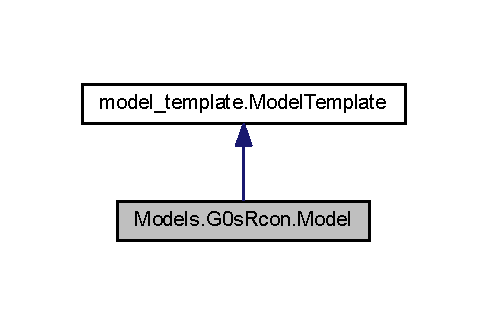
\includegraphics[width=234pt]{class_models_1_1_g0s_rcon_1_1_model__inherit__graph}
\end{center}
\end{figure}


Collaboration diagram for Models.\-G0s\-Rcon.\-Model\-:
\nopagebreak
\begin{figure}[H]
\begin{center}
\leavevmode
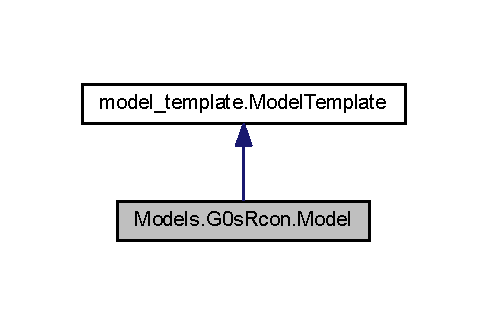
\includegraphics[width=234pt]{class_models_1_1_g0s_rcon_1_1_model__coll__graph}
\end{center}
\end{figure}
\subsection*{Public Member Functions}
\begin{DoxyCompactItemize}
\item 
def \hyperlink{class_models_1_1_g0s_rcon_1_1_model_a75577cbd55530984550f172e80875b8e}{\-\_\-\-\_\-init\-\_\-\-\_\-}
\item 
def \hyperlink{class_models_1_1_g0s_rcon_1_1_model_a6efae20699b0011357265ea89c81fba3}{calc\-\_\-b\-\_\-h\-\_\-vi}
\item 
def \hyperlink{class_models_1_1_g0s_rcon_1_1_model_a04ecbecf6f7290a70654271eabd576e4}{calc\-\_\-b\-\_\-h}
\item 
def \hyperlink{class_models_1_1_g0s_rcon_1_1_model_aff984472f5f2fa388212fbc3cc93b3ce}{calc\-\_\-phi\-\_\-hvi}
\item 
def \hyperlink{class_models_1_1_g0s_rcon_1_1_model_abf05f96a51cb09f5a59a6e0d7ad1d62f}{calc\-\_\-\-P\-\_\-h\-\_\-vi}
\item 
def \hyperlink{class_models_1_1_g0s_rcon_1_1_model_ac8288b22f43428b485bae414a5f187f7}{calc\-\_\-r\-\_\-vi}
\item 
def \hyperlink{class_models_1_1_g0s_rcon_1_1_model_ab4d9e1ac6366938dc1ef8e3eabccc039}{calc\-\_\-\-S\-\_\-vi}
\item 
def \hyperlink{class_models_1_1_g0s_rcon_1_1_model_a7d652f6c1837279cb8b2478cf22149dd}{calc\-\_\-gamma\-\_\-vi}
\end{DoxyCompactItemize}
\subsection*{Additional Inherited Members}


\subsection{Detailed Description}
\begin{DoxyVerb}Modelo\end{DoxyVerb}
 

\subsection{Constructor \& Destructor Documentation}
\hypertarget{class_models_1_1_g0s_rcon_1_1_model_a75577cbd55530984550f172e80875b8e}{\index{Models\-::\-G0s\-Rcon\-::\-Model@{Models\-::\-G0s\-Rcon\-::\-Model}!\-\_\-\-\_\-init\-\_\-\-\_\-@{\-\_\-\-\_\-init\-\_\-\-\_\-}}
\index{\-\_\-\-\_\-init\-\_\-\-\_\-@{\-\_\-\-\_\-init\-\_\-\-\_\-}!Models::G0sRcon::Model@{Models\-::\-G0s\-Rcon\-::\-Model}}
\subsubsection[{\-\_\-\-\_\-init\-\_\-\-\_\-}]{\setlength{\rightskip}{0pt plus 5cm}def Models.\-G0s\-Rcon.\-Model.\-\_\-\-\_\-init\-\_\-\-\_\- (
\begin{DoxyParamCaption}
\item[{}]{self, }
\item[{}]{model\-Name}
\end{DoxyParamCaption}
)}}\label{class_models_1_1_g0s_rcon_1_1_model_a75577cbd55530984550f172e80875b8e}


\subsection{Member Function Documentation}
\hypertarget{class_models_1_1_g0s_rcon_1_1_model_a04ecbecf6f7290a70654271eabd576e4}{\index{Models\-::\-G0s\-Rcon\-::\-Model@{Models\-::\-G0s\-Rcon\-::\-Model}!calc\-\_\-b\-\_\-h@{calc\-\_\-b\-\_\-h}}
\index{calc\-\_\-b\-\_\-h@{calc\-\_\-b\-\_\-h}!Models::G0sRcon::Model@{Models\-::\-G0s\-Rcon\-::\-Model}}
\subsubsection[{calc\-\_\-b\-\_\-h}]{\setlength{\rightskip}{0pt plus 5cm}def Models.\-G0s\-Rcon.\-Model.\-calc\-\_\-b\-\_\-h (
\begin{DoxyParamCaption}
\item[{}]{self, }
\item[{}]{dm, }
\item[{}]{t}
\end{DoxyParamCaption}
)}}\label{class_models_1_1_g0s_rcon_1_1_model_a04ecbecf6f7290a70654271eabd576e4}
\hypertarget{class_models_1_1_g0s_rcon_1_1_model_a6efae20699b0011357265ea89c81fba3}{\index{Models\-::\-G0s\-Rcon\-::\-Model@{Models\-::\-G0s\-Rcon\-::\-Model}!calc\-\_\-b\-\_\-h\-\_\-vi@{calc\-\_\-b\-\_\-h\-\_\-vi}}
\index{calc\-\_\-b\-\_\-h\-\_\-vi@{calc\-\_\-b\-\_\-h\-\_\-vi}!Models::G0sRcon::Model@{Models\-::\-G0s\-Rcon\-::\-Model}}
\subsubsection[{calc\-\_\-b\-\_\-h\-\_\-vi}]{\setlength{\rightskip}{0pt plus 5cm}def Models.\-G0s\-Rcon.\-Model.\-calc\-\_\-b\-\_\-h\-\_\-vi (
\begin{DoxyParamCaption}
\item[{}]{self, }
\item[{}]{dm, }
\item[{}]{t}
\end{DoxyParamCaption}
)}}\label{class_models_1_1_g0s_rcon_1_1_model_a6efae20699b0011357265ea89c81fba3}
\hypertarget{class_models_1_1_g0s_rcon_1_1_model_a7d652f6c1837279cb8b2478cf22149dd}{\index{Models\-::\-G0s\-Rcon\-::\-Model@{Models\-::\-G0s\-Rcon\-::\-Model}!calc\-\_\-gamma\-\_\-vi@{calc\-\_\-gamma\-\_\-vi}}
\index{calc\-\_\-gamma\-\_\-vi@{calc\-\_\-gamma\-\_\-vi}!Models::G0sRcon::Model@{Models\-::\-G0s\-Rcon\-::\-Model}}
\subsubsection[{calc\-\_\-gamma\-\_\-vi}]{\setlength{\rightskip}{0pt plus 5cm}def Models.\-G0s\-Rcon.\-Model.\-calc\-\_\-gamma\-\_\-vi (
\begin{DoxyParamCaption}
\item[{}]{self, }
\item[{}]{dm, }
\item[{}]{t}
\end{DoxyParamCaption}
)}}\label{class_models_1_1_g0s_rcon_1_1_model_a7d652f6c1837279cb8b2478cf22149dd}
\hypertarget{class_models_1_1_g0s_rcon_1_1_model_abf05f96a51cb09f5a59a6e0d7ad1d62f}{\index{Models\-::\-G0s\-Rcon\-::\-Model@{Models\-::\-G0s\-Rcon\-::\-Model}!calc\-\_\-\-P\-\_\-h\-\_\-vi@{calc\-\_\-\-P\-\_\-h\-\_\-vi}}
\index{calc\-\_\-\-P\-\_\-h\-\_\-vi@{calc\-\_\-\-P\-\_\-h\-\_\-vi}!Models::G0sRcon::Model@{Models\-::\-G0s\-Rcon\-::\-Model}}
\subsubsection[{calc\-\_\-\-P\-\_\-h\-\_\-vi}]{\setlength{\rightskip}{0pt plus 5cm}def Models.\-G0s\-Rcon.\-Model.\-calc\-\_\-\-P\-\_\-h\-\_\-vi (
\begin{DoxyParamCaption}
\item[{}]{self, }
\item[{}]{dm, }
\item[{}]{t}
\end{DoxyParamCaption}
)}}\label{class_models_1_1_g0s_rcon_1_1_model_abf05f96a51cb09f5a59a6e0d7ad1d62f}
\hypertarget{class_models_1_1_g0s_rcon_1_1_model_aff984472f5f2fa388212fbc3cc93b3ce}{\index{Models\-::\-G0s\-Rcon\-::\-Model@{Models\-::\-G0s\-Rcon\-::\-Model}!calc\-\_\-phi\-\_\-hvi@{calc\-\_\-phi\-\_\-hvi}}
\index{calc\-\_\-phi\-\_\-hvi@{calc\-\_\-phi\-\_\-hvi}!Models::G0sRcon::Model@{Models\-::\-G0s\-Rcon\-::\-Model}}
\subsubsection[{calc\-\_\-phi\-\_\-hvi}]{\setlength{\rightskip}{0pt plus 5cm}def Models.\-G0s\-Rcon.\-Model.\-calc\-\_\-phi\-\_\-hvi (
\begin{DoxyParamCaption}
\item[{}]{self, }
\item[{}]{dm, }
\item[{}]{t}
\end{DoxyParamCaption}
)}}\label{class_models_1_1_g0s_rcon_1_1_model_aff984472f5f2fa388212fbc3cc93b3ce}
\hypertarget{class_models_1_1_g0s_rcon_1_1_model_ac8288b22f43428b485bae414a5f187f7}{\index{Models\-::\-G0s\-Rcon\-::\-Model@{Models\-::\-G0s\-Rcon\-::\-Model}!calc\-\_\-r\-\_\-vi@{calc\-\_\-r\-\_\-vi}}
\index{calc\-\_\-r\-\_\-vi@{calc\-\_\-r\-\_\-vi}!Models::G0sRcon::Model@{Models\-::\-G0s\-Rcon\-::\-Model}}
\subsubsection[{calc\-\_\-r\-\_\-vi}]{\setlength{\rightskip}{0pt plus 5cm}def Models.\-G0s\-Rcon.\-Model.\-calc\-\_\-r\-\_\-vi (
\begin{DoxyParamCaption}
\item[{}]{self, }
\item[{}]{dm, }
\item[{}]{t}
\end{DoxyParamCaption}
)}}\label{class_models_1_1_g0s_rcon_1_1_model_ac8288b22f43428b485bae414a5f187f7}
\hypertarget{class_models_1_1_g0s_rcon_1_1_model_ab4d9e1ac6366938dc1ef8e3eabccc039}{\index{Models\-::\-G0s\-Rcon\-::\-Model@{Models\-::\-G0s\-Rcon\-::\-Model}!calc\-\_\-\-S\-\_\-vi@{calc\-\_\-\-S\-\_\-vi}}
\index{calc\-\_\-\-S\-\_\-vi@{calc\-\_\-\-S\-\_\-vi}!Models::G0sRcon::Model@{Models\-::\-G0s\-Rcon\-::\-Model}}
\subsubsection[{calc\-\_\-\-S\-\_\-vi}]{\setlength{\rightskip}{0pt plus 5cm}def Models.\-G0s\-Rcon.\-Model.\-calc\-\_\-\-S\-\_\-vi (
\begin{DoxyParamCaption}
\item[{}]{self, }
\item[{}]{dm, }
\item[{}]{t}
\end{DoxyParamCaption}
)}}\label{class_models_1_1_g0s_rcon_1_1_model_ab4d9e1ac6366938dc1ef8e3eabccc039}


The documentation for this class was generated from the following file\-:\begin{DoxyCompactItemize}
\item 
Models/\hyperlink{_g0s_rcon_8py}{G0s\-Rcon.\-py}\end{DoxyCompactItemize}

\hypertarget{class_models_1_1_gqs_r_1_1_model}{\section{Models.\-Gqs\-R.\-Model Class Reference}
\label{class_models_1_1_gqs_r_1_1_model}\index{Models.\-Gqs\-R.\-Model@{Models.\-Gqs\-R.\-Model}}
}


Inheritance diagram for Models.\-Gqs\-R.\-Model\-:
\nopagebreak
\begin{figure}[H]
\begin{center}
\leavevmode
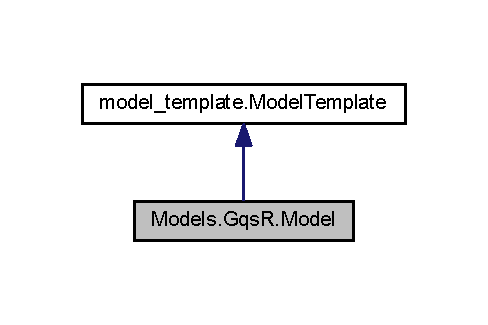
\includegraphics[width=234pt]{class_models_1_1_gqs_r_1_1_model__inherit__graph}
\end{center}
\end{figure}


Collaboration diagram for Models.\-Gqs\-R.\-Model\-:
\nopagebreak
\begin{figure}[H]
\begin{center}
\leavevmode
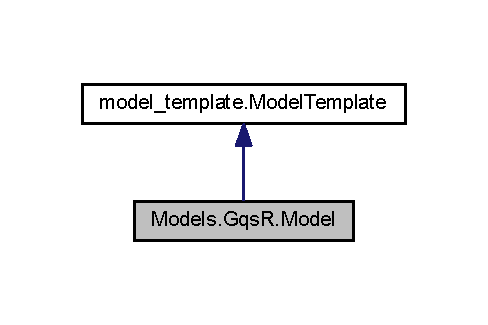
\includegraphics[width=234pt]{class_models_1_1_gqs_r_1_1_model__coll__graph}
\end{center}
\end{figure}
\subsection*{Public Member Functions}
\begin{DoxyCompactItemize}
\item 
def \hyperlink{class_models_1_1_gqs_r_1_1_model_ab9569b7d0438c79e41e1457a81b472f3}{\-\_\-\-\_\-init\-\_\-\-\_\-}
\item 
def \hyperlink{class_models_1_1_gqs_r_1_1_model_ab571f238a67be01432388c872597338e}{calc\-\_\-b\-\_\-h\-\_\-vi}
\item 
def \hyperlink{class_models_1_1_gqs_r_1_1_model_a7930f48b5f56668c1c967278e26c5272}{calc\-\_\-b\-\_\-h}
\item 
def \hyperlink{class_models_1_1_gqs_r_1_1_model_a98add83363838690c7a06cd8f0b5d775}{calc\-\_\-\-P\-\_\-h\-\_\-vi}
\item 
def \hyperlink{class_models_1_1_gqs_r_1_1_model_aa33e1c03ab2aff8ac89d8ccff9431dd1}{calc\-\_\-r\-\_\-vi}
\item 
def \hyperlink{class_models_1_1_gqs_r_1_1_model_aa298eed276b77a4acea8a3418cef7209}{calc\-\_\-\-S\-\_\-vi}
\item 
def \hyperlink{class_models_1_1_gqs_r_1_1_model_a30c28172c622d3edb07272ae4b2c61f0}{calc\-\_\-gamma\-\_\-vi}
\end{DoxyCompactItemize}
\subsection*{Additional Inherited Members}


\subsection{Detailed Description}
\begin{DoxyVerb}Modelo\end{DoxyVerb}
 

\subsection{Constructor \& Destructor Documentation}
\hypertarget{class_models_1_1_gqs_r_1_1_model_ab9569b7d0438c79e41e1457a81b472f3}{\index{Models\-::\-Gqs\-R\-::\-Model@{Models\-::\-Gqs\-R\-::\-Model}!\-\_\-\-\_\-init\-\_\-\-\_\-@{\-\_\-\-\_\-init\-\_\-\-\_\-}}
\index{\-\_\-\-\_\-init\-\_\-\-\_\-@{\-\_\-\-\_\-init\-\_\-\-\_\-}!Models::GqsR::Model@{Models\-::\-Gqs\-R\-::\-Model}}
\subsubsection[{\-\_\-\-\_\-init\-\_\-\-\_\-}]{\setlength{\rightskip}{0pt plus 5cm}def Models.\-Gqs\-R.\-Model.\-\_\-\-\_\-init\-\_\-\-\_\- (
\begin{DoxyParamCaption}
\item[{}]{self, }
\item[{}]{model\-Name}
\end{DoxyParamCaption}
)}}\label{class_models_1_1_gqs_r_1_1_model_ab9569b7d0438c79e41e1457a81b472f3}


\subsection{Member Function Documentation}
\hypertarget{class_models_1_1_gqs_r_1_1_model_a7930f48b5f56668c1c967278e26c5272}{\index{Models\-::\-Gqs\-R\-::\-Model@{Models\-::\-Gqs\-R\-::\-Model}!calc\-\_\-b\-\_\-h@{calc\-\_\-b\-\_\-h}}
\index{calc\-\_\-b\-\_\-h@{calc\-\_\-b\-\_\-h}!Models::GqsR::Model@{Models\-::\-Gqs\-R\-::\-Model}}
\subsubsection[{calc\-\_\-b\-\_\-h}]{\setlength{\rightskip}{0pt plus 5cm}def Models.\-Gqs\-R.\-Model.\-calc\-\_\-b\-\_\-h (
\begin{DoxyParamCaption}
\item[{}]{self, }
\item[{}]{dm, }
\item[{}]{t}
\end{DoxyParamCaption}
)}}\label{class_models_1_1_gqs_r_1_1_model_a7930f48b5f56668c1c967278e26c5272}
\hypertarget{class_models_1_1_gqs_r_1_1_model_ab571f238a67be01432388c872597338e}{\index{Models\-::\-Gqs\-R\-::\-Model@{Models\-::\-Gqs\-R\-::\-Model}!calc\-\_\-b\-\_\-h\-\_\-vi@{calc\-\_\-b\-\_\-h\-\_\-vi}}
\index{calc\-\_\-b\-\_\-h\-\_\-vi@{calc\-\_\-b\-\_\-h\-\_\-vi}!Models::GqsR::Model@{Models\-::\-Gqs\-R\-::\-Model}}
\subsubsection[{calc\-\_\-b\-\_\-h\-\_\-vi}]{\setlength{\rightskip}{0pt plus 5cm}def Models.\-Gqs\-R.\-Model.\-calc\-\_\-b\-\_\-h\-\_\-vi (
\begin{DoxyParamCaption}
\item[{}]{self, }
\item[{}]{dm, }
\item[{}]{t}
\end{DoxyParamCaption}
)}}\label{class_models_1_1_gqs_r_1_1_model_ab571f238a67be01432388c872597338e}
\hypertarget{class_models_1_1_gqs_r_1_1_model_a30c28172c622d3edb07272ae4b2c61f0}{\index{Models\-::\-Gqs\-R\-::\-Model@{Models\-::\-Gqs\-R\-::\-Model}!calc\-\_\-gamma\-\_\-vi@{calc\-\_\-gamma\-\_\-vi}}
\index{calc\-\_\-gamma\-\_\-vi@{calc\-\_\-gamma\-\_\-vi}!Models::GqsR::Model@{Models\-::\-Gqs\-R\-::\-Model}}
\subsubsection[{calc\-\_\-gamma\-\_\-vi}]{\setlength{\rightskip}{0pt plus 5cm}def Models.\-Gqs\-R.\-Model.\-calc\-\_\-gamma\-\_\-vi (
\begin{DoxyParamCaption}
\item[{}]{self, }
\item[{}]{dm, }
\item[{}]{t}
\end{DoxyParamCaption}
)}}\label{class_models_1_1_gqs_r_1_1_model_a30c28172c622d3edb07272ae4b2c61f0}
\hypertarget{class_models_1_1_gqs_r_1_1_model_a98add83363838690c7a06cd8f0b5d775}{\index{Models\-::\-Gqs\-R\-::\-Model@{Models\-::\-Gqs\-R\-::\-Model}!calc\-\_\-\-P\-\_\-h\-\_\-vi@{calc\-\_\-\-P\-\_\-h\-\_\-vi}}
\index{calc\-\_\-\-P\-\_\-h\-\_\-vi@{calc\-\_\-\-P\-\_\-h\-\_\-vi}!Models::GqsR::Model@{Models\-::\-Gqs\-R\-::\-Model}}
\subsubsection[{calc\-\_\-\-P\-\_\-h\-\_\-vi}]{\setlength{\rightskip}{0pt plus 5cm}def Models.\-Gqs\-R.\-Model.\-calc\-\_\-\-P\-\_\-h\-\_\-vi (
\begin{DoxyParamCaption}
\item[{}]{self, }
\item[{}]{dm, }
\item[{}]{t}
\end{DoxyParamCaption}
)}}\label{class_models_1_1_gqs_r_1_1_model_a98add83363838690c7a06cd8f0b5d775}
\hypertarget{class_models_1_1_gqs_r_1_1_model_aa33e1c03ab2aff8ac89d8ccff9431dd1}{\index{Models\-::\-Gqs\-R\-::\-Model@{Models\-::\-Gqs\-R\-::\-Model}!calc\-\_\-r\-\_\-vi@{calc\-\_\-r\-\_\-vi}}
\index{calc\-\_\-r\-\_\-vi@{calc\-\_\-r\-\_\-vi}!Models::GqsR::Model@{Models\-::\-Gqs\-R\-::\-Model}}
\subsubsection[{calc\-\_\-r\-\_\-vi}]{\setlength{\rightskip}{0pt plus 5cm}def Models.\-Gqs\-R.\-Model.\-calc\-\_\-r\-\_\-vi (
\begin{DoxyParamCaption}
\item[{}]{self, }
\item[{}]{dm, }
\item[{}]{t}
\end{DoxyParamCaption}
)}}\label{class_models_1_1_gqs_r_1_1_model_aa33e1c03ab2aff8ac89d8ccff9431dd1}
\hypertarget{class_models_1_1_gqs_r_1_1_model_aa298eed276b77a4acea8a3418cef7209}{\index{Models\-::\-Gqs\-R\-::\-Model@{Models\-::\-Gqs\-R\-::\-Model}!calc\-\_\-\-S\-\_\-vi@{calc\-\_\-\-S\-\_\-vi}}
\index{calc\-\_\-\-S\-\_\-vi@{calc\-\_\-\-S\-\_\-vi}!Models::GqsR::Model@{Models\-::\-Gqs\-R\-::\-Model}}
\subsubsection[{calc\-\_\-\-S\-\_\-vi}]{\setlength{\rightskip}{0pt plus 5cm}def Models.\-Gqs\-R.\-Model.\-calc\-\_\-\-S\-\_\-vi (
\begin{DoxyParamCaption}
\item[{}]{self, }
\item[{}]{dm, }
\item[{}]{t}
\end{DoxyParamCaption}
)}}\label{class_models_1_1_gqs_r_1_1_model_aa298eed276b77a4acea8a3418cef7209}


The documentation for this class was generated from the following file\-:\begin{DoxyCompactItemize}
\item 
Models/\hyperlink{_gqs_r_8py}{Gqs\-R.\-py}\end{DoxyCompactItemize}

\hypertarget{class_models_1_1_g0s_r_1_1_model}{\section{Models.\-G0s\-R.\-Model Class Reference}
\label{class_models_1_1_g0s_r_1_1_model}\index{Models.\-G0s\-R.\-Model@{Models.\-G0s\-R.\-Model}}
}


Inheritance diagram for Models.\-G0s\-R.\-Model\-:
\nopagebreak
\begin{figure}[H]
\begin{center}
\leavevmode
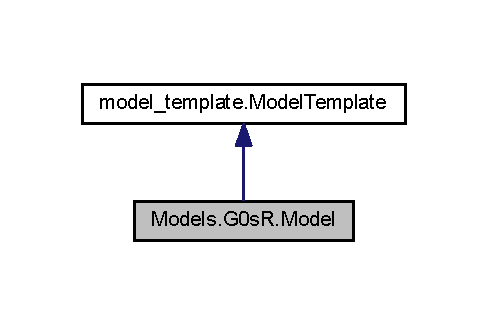
\includegraphics[width=234pt]{class_models_1_1_g0s_r_1_1_model__inherit__graph}
\end{center}
\end{figure}


Collaboration diagram for Models.\-G0s\-R.\-Model\-:
\nopagebreak
\begin{figure}[H]
\begin{center}
\leavevmode
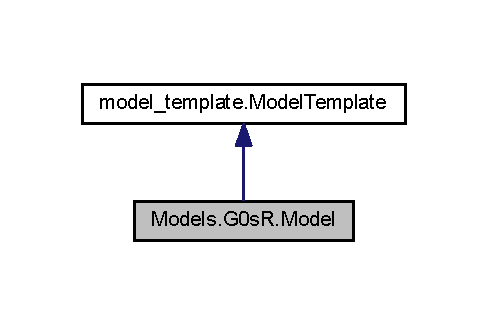
\includegraphics[width=234pt]{class_models_1_1_g0s_r_1_1_model__coll__graph}
\end{center}
\end{figure}
\subsection*{Public Member Functions}
\begin{DoxyCompactItemize}
\item 
def \hyperlink{class_models_1_1_g0s_r_1_1_model_a7e10b2901bfa6623d9816dab90f35e07}{\-\_\-\-\_\-init\-\_\-\-\_\-}
\item 
def \hyperlink{class_models_1_1_g0s_r_1_1_model_af98cbbfa8a7b918619a3bec7768c92c3}{calc\-\_\-b\-\_\-h\-\_\-vi}
\item 
def \hyperlink{class_models_1_1_g0s_r_1_1_model_a0973c82a818d91cfe1bc52020b774311}{calc\-\_\-b\-\_\-h}
\item 
def \hyperlink{class_models_1_1_g0s_r_1_1_model_a4f64771a7138fd15cbdb262f1eca0b68}{calc\-\_\-\-P\-\_\-h\-\_\-vi}
\item 
def \hyperlink{class_models_1_1_g0s_r_1_1_model_ad366c74ec566a8771fe979225c98becb}{calc\-\_\-r\-\_\-vi}
\item 
def \hyperlink{class_models_1_1_g0s_r_1_1_model_adf189ac478321a40826a06ddcf099c49}{calc\-\_\-\-S\-\_\-vi}
\item 
def \hyperlink{class_models_1_1_g0s_r_1_1_model_aa112b53db6ae1a9ccbceaf59eb83d85e}{calc\-\_\-gamma\-\_\-vi}
\end{DoxyCompactItemize}
\subsection*{Additional Inherited Members}


\subsection{Detailed Description}
\begin{DoxyVerb}Modelo\end{DoxyVerb}
 

\subsection{Constructor \& Destructor Documentation}
\hypertarget{class_models_1_1_g0s_r_1_1_model_a7e10b2901bfa6623d9816dab90f35e07}{\index{Models\-::\-G0s\-R\-::\-Model@{Models\-::\-G0s\-R\-::\-Model}!\-\_\-\-\_\-init\-\_\-\-\_\-@{\-\_\-\-\_\-init\-\_\-\-\_\-}}
\index{\-\_\-\-\_\-init\-\_\-\-\_\-@{\-\_\-\-\_\-init\-\_\-\-\_\-}!Models::G0sR::Model@{Models\-::\-G0s\-R\-::\-Model}}
\subsubsection[{\-\_\-\-\_\-init\-\_\-\-\_\-}]{\setlength{\rightskip}{0pt plus 5cm}def Models.\-G0s\-R.\-Model.\-\_\-\-\_\-init\-\_\-\-\_\- (
\begin{DoxyParamCaption}
\item[{}]{self, }
\item[{}]{model\-Name}
\end{DoxyParamCaption}
)}}\label{class_models_1_1_g0s_r_1_1_model_a7e10b2901bfa6623d9816dab90f35e07}


\subsection{Member Function Documentation}
\hypertarget{class_models_1_1_g0s_r_1_1_model_a0973c82a818d91cfe1bc52020b774311}{\index{Models\-::\-G0s\-R\-::\-Model@{Models\-::\-G0s\-R\-::\-Model}!calc\-\_\-b\-\_\-h@{calc\-\_\-b\-\_\-h}}
\index{calc\-\_\-b\-\_\-h@{calc\-\_\-b\-\_\-h}!Models::G0sR::Model@{Models\-::\-G0s\-R\-::\-Model}}
\subsubsection[{calc\-\_\-b\-\_\-h}]{\setlength{\rightskip}{0pt plus 5cm}def Models.\-G0s\-R.\-Model.\-calc\-\_\-b\-\_\-h (
\begin{DoxyParamCaption}
\item[{}]{self, }
\item[{}]{dm, }
\item[{}]{t}
\end{DoxyParamCaption}
)}}\label{class_models_1_1_g0s_r_1_1_model_a0973c82a818d91cfe1bc52020b774311}
\hypertarget{class_models_1_1_g0s_r_1_1_model_af98cbbfa8a7b918619a3bec7768c92c3}{\index{Models\-::\-G0s\-R\-::\-Model@{Models\-::\-G0s\-R\-::\-Model}!calc\-\_\-b\-\_\-h\-\_\-vi@{calc\-\_\-b\-\_\-h\-\_\-vi}}
\index{calc\-\_\-b\-\_\-h\-\_\-vi@{calc\-\_\-b\-\_\-h\-\_\-vi}!Models::G0sR::Model@{Models\-::\-G0s\-R\-::\-Model}}
\subsubsection[{calc\-\_\-b\-\_\-h\-\_\-vi}]{\setlength{\rightskip}{0pt plus 5cm}def Models.\-G0s\-R.\-Model.\-calc\-\_\-b\-\_\-h\-\_\-vi (
\begin{DoxyParamCaption}
\item[{}]{self, }
\item[{}]{dm, }
\item[{}]{t}
\end{DoxyParamCaption}
)}}\label{class_models_1_1_g0s_r_1_1_model_af98cbbfa8a7b918619a3bec7768c92c3}
\hypertarget{class_models_1_1_g0s_r_1_1_model_aa112b53db6ae1a9ccbceaf59eb83d85e}{\index{Models\-::\-G0s\-R\-::\-Model@{Models\-::\-G0s\-R\-::\-Model}!calc\-\_\-gamma\-\_\-vi@{calc\-\_\-gamma\-\_\-vi}}
\index{calc\-\_\-gamma\-\_\-vi@{calc\-\_\-gamma\-\_\-vi}!Models::G0sR::Model@{Models\-::\-G0s\-R\-::\-Model}}
\subsubsection[{calc\-\_\-gamma\-\_\-vi}]{\setlength{\rightskip}{0pt plus 5cm}def Models.\-G0s\-R.\-Model.\-calc\-\_\-gamma\-\_\-vi (
\begin{DoxyParamCaption}
\item[{}]{self, }
\item[{}]{dm, }
\item[{}]{t}
\end{DoxyParamCaption}
)}}\label{class_models_1_1_g0s_r_1_1_model_aa112b53db6ae1a9ccbceaf59eb83d85e}
\hypertarget{class_models_1_1_g0s_r_1_1_model_a4f64771a7138fd15cbdb262f1eca0b68}{\index{Models\-::\-G0s\-R\-::\-Model@{Models\-::\-G0s\-R\-::\-Model}!calc\-\_\-\-P\-\_\-h\-\_\-vi@{calc\-\_\-\-P\-\_\-h\-\_\-vi}}
\index{calc\-\_\-\-P\-\_\-h\-\_\-vi@{calc\-\_\-\-P\-\_\-h\-\_\-vi}!Models::G0sR::Model@{Models\-::\-G0s\-R\-::\-Model}}
\subsubsection[{calc\-\_\-\-P\-\_\-h\-\_\-vi}]{\setlength{\rightskip}{0pt plus 5cm}def Models.\-G0s\-R.\-Model.\-calc\-\_\-\-P\-\_\-h\-\_\-vi (
\begin{DoxyParamCaption}
\item[{}]{self, }
\item[{}]{dm, }
\item[{}]{t}
\end{DoxyParamCaption}
)}}\label{class_models_1_1_g0s_r_1_1_model_a4f64771a7138fd15cbdb262f1eca0b68}
\hypertarget{class_models_1_1_g0s_r_1_1_model_ad366c74ec566a8771fe979225c98becb}{\index{Models\-::\-G0s\-R\-::\-Model@{Models\-::\-G0s\-R\-::\-Model}!calc\-\_\-r\-\_\-vi@{calc\-\_\-r\-\_\-vi}}
\index{calc\-\_\-r\-\_\-vi@{calc\-\_\-r\-\_\-vi}!Models::G0sR::Model@{Models\-::\-G0s\-R\-::\-Model}}
\subsubsection[{calc\-\_\-r\-\_\-vi}]{\setlength{\rightskip}{0pt plus 5cm}def Models.\-G0s\-R.\-Model.\-calc\-\_\-r\-\_\-vi (
\begin{DoxyParamCaption}
\item[{}]{self, }
\item[{}]{dm, }
\item[{}]{t}
\end{DoxyParamCaption}
)}}\label{class_models_1_1_g0s_r_1_1_model_ad366c74ec566a8771fe979225c98becb}
\hypertarget{class_models_1_1_g0s_r_1_1_model_adf189ac478321a40826a06ddcf099c49}{\index{Models\-::\-G0s\-R\-::\-Model@{Models\-::\-G0s\-R\-::\-Model}!calc\-\_\-\-S\-\_\-vi@{calc\-\_\-\-S\-\_\-vi}}
\index{calc\-\_\-\-S\-\_\-vi@{calc\-\_\-\-S\-\_\-vi}!Models::G0sR::Model@{Models\-::\-G0s\-R\-::\-Model}}
\subsubsection[{calc\-\_\-\-S\-\_\-vi}]{\setlength{\rightskip}{0pt plus 5cm}def Models.\-G0s\-R.\-Model.\-calc\-\_\-\-S\-\_\-vi (
\begin{DoxyParamCaption}
\item[{}]{self, }
\item[{}]{dm, }
\item[{}]{t}
\end{DoxyParamCaption}
)}}\label{class_models_1_1_g0s_r_1_1_model_adf189ac478321a40826a06ddcf099c49}


The documentation for this class was generated from the following file\-:\begin{DoxyCompactItemize}
\item 
Models/\hyperlink{_g0s_r_8py}{G0s\-R.\-py}\end{DoxyCompactItemize}

\hypertarget{class_models_1_1_g0s_1_1_model}{\section{Models.\-G0s.\-Model Class Reference}
\label{class_models_1_1_g0s_1_1_model}\index{Models.\-G0s.\-Model@{Models.\-G0s.\-Model}}
}


Inheritance diagram for Models.\-G0s.\-Model\-:
\nopagebreak
\begin{figure}[H]
\begin{center}
\leavevmode
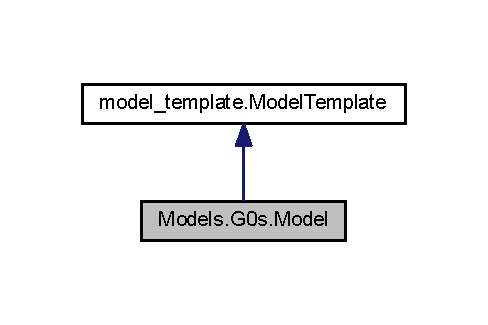
\includegraphics[width=234pt]{class_models_1_1_g0s_1_1_model__inherit__graph}
\end{center}
\end{figure}


Collaboration diagram for Models.\-G0s.\-Model\-:
\nopagebreak
\begin{figure}[H]
\begin{center}
\leavevmode
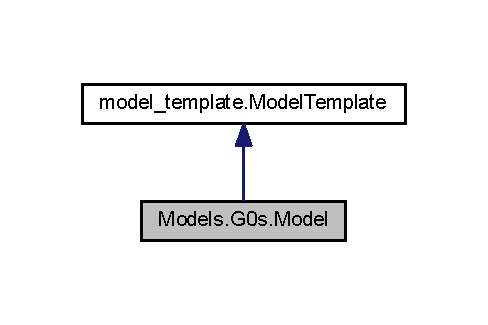
\includegraphics[width=234pt]{class_models_1_1_g0s_1_1_model__coll__graph}
\end{center}
\end{figure}
\subsection*{Public Member Functions}
\begin{DoxyCompactItemize}
\item 
def \hyperlink{class_models_1_1_g0s_1_1_model_a9de95124847058da5de0b08ec9bbf389}{\-\_\-\-\_\-init\-\_\-\-\_\-}
\item 
def \hyperlink{class_models_1_1_g0s_1_1_model_ae3c510b8766285dd9adc1e219cce4783}{calc\-\_\-b\-\_\-h\-\_\-vi}
\item 
def \hyperlink{class_models_1_1_g0s_1_1_model_af033fa0a5545ad8a179c9d1a2e47605c}{calc\-\_\-b\-\_\-h}
\item 
def \hyperlink{class_models_1_1_g0s_1_1_model_adc2d5d377d647fe917a092e3ca78d285}{calc\-\_\-\-P\-\_\-h\-\_\-vi}
\item 
def \hyperlink{class_models_1_1_g0s_1_1_model_a3cef5601fddac0a3c0dc92bc97cca248}{calc\-\_\-r\-\_\-vi}
\item 
def \hyperlink{class_models_1_1_g0s_1_1_model_a88b8bd82470861d8a56c8c7c082b13ab}{calc\-\_\-\-S\-\_\-vi}
\end{DoxyCompactItemize}
\subsection*{Additional Inherited Members}


\subsection{Detailed Description}
\begin{DoxyVerb}Modelo\end{DoxyVerb}
 

\subsection{Constructor \& Destructor Documentation}
\hypertarget{class_models_1_1_g0s_1_1_model_a9de95124847058da5de0b08ec9bbf389}{\index{Models\-::\-G0s\-::\-Model@{Models\-::\-G0s\-::\-Model}!\-\_\-\-\_\-init\-\_\-\-\_\-@{\-\_\-\-\_\-init\-\_\-\-\_\-}}
\index{\-\_\-\-\_\-init\-\_\-\-\_\-@{\-\_\-\-\_\-init\-\_\-\-\_\-}!Models::G0s::Model@{Models\-::\-G0s\-::\-Model}}
\subsubsection[{\-\_\-\-\_\-init\-\_\-\-\_\-}]{\setlength{\rightskip}{0pt plus 5cm}def Models.\-G0s.\-Model.\-\_\-\-\_\-init\-\_\-\-\_\- (
\begin{DoxyParamCaption}
\item[{}]{self, }
\item[{}]{model\-Name}
\end{DoxyParamCaption}
)}}\label{class_models_1_1_g0s_1_1_model_a9de95124847058da5de0b08ec9bbf389}


\subsection{Member Function Documentation}
\hypertarget{class_models_1_1_g0s_1_1_model_af033fa0a5545ad8a179c9d1a2e47605c}{\index{Models\-::\-G0s\-::\-Model@{Models\-::\-G0s\-::\-Model}!calc\-\_\-b\-\_\-h@{calc\-\_\-b\-\_\-h}}
\index{calc\-\_\-b\-\_\-h@{calc\-\_\-b\-\_\-h}!Models::G0s::Model@{Models\-::\-G0s\-::\-Model}}
\subsubsection[{calc\-\_\-b\-\_\-h}]{\setlength{\rightskip}{0pt plus 5cm}def Models.\-G0s.\-Model.\-calc\-\_\-b\-\_\-h (
\begin{DoxyParamCaption}
\item[{}]{self, }
\item[{}]{dm, }
\item[{}]{t}
\end{DoxyParamCaption}
)}}\label{class_models_1_1_g0s_1_1_model_af033fa0a5545ad8a179c9d1a2e47605c}
\hypertarget{class_models_1_1_g0s_1_1_model_ae3c510b8766285dd9adc1e219cce4783}{\index{Models\-::\-G0s\-::\-Model@{Models\-::\-G0s\-::\-Model}!calc\-\_\-b\-\_\-h\-\_\-vi@{calc\-\_\-b\-\_\-h\-\_\-vi}}
\index{calc\-\_\-b\-\_\-h\-\_\-vi@{calc\-\_\-b\-\_\-h\-\_\-vi}!Models::G0s::Model@{Models\-::\-G0s\-::\-Model}}
\subsubsection[{calc\-\_\-b\-\_\-h\-\_\-vi}]{\setlength{\rightskip}{0pt plus 5cm}def Models.\-G0s.\-Model.\-calc\-\_\-b\-\_\-h\-\_\-vi (
\begin{DoxyParamCaption}
\item[{}]{self, }
\item[{}]{dm, }
\item[{}]{t}
\end{DoxyParamCaption}
)}}\label{class_models_1_1_g0s_1_1_model_ae3c510b8766285dd9adc1e219cce4783}
\hypertarget{class_models_1_1_g0s_1_1_model_adc2d5d377d647fe917a092e3ca78d285}{\index{Models\-::\-G0s\-::\-Model@{Models\-::\-G0s\-::\-Model}!calc\-\_\-\-P\-\_\-h\-\_\-vi@{calc\-\_\-\-P\-\_\-h\-\_\-vi}}
\index{calc\-\_\-\-P\-\_\-h\-\_\-vi@{calc\-\_\-\-P\-\_\-h\-\_\-vi}!Models::G0s::Model@{Models\-::\-G0s\-::\-Model}}
\subsubsection[{calc\-\_\-\-P\-\_\-h\-\_\-vi}]{\setlength{\rightskip}{0pt plus 5cm}def Models.\-G0s.\-Model.\-calc\-\_\-\-P\-\_\-h\-\_\-vi (
\begin{DoxyParamCaption}
\item[{}]{self, }
\item[{}]{dm, }
\item[{}]{t}
\end{DoxyParamCaption}
)}}\label{class_models_1_1_g0s_1_1_model_adc2d5d377d647fe917a092e3ca78d285}
\hypertarget{class_models_1_1_g0s_1_1_model_a3cef5601fddac0a3c0dc92bc97cca248}{\index{Models\-::\-G0s\-::\-Model@{Models\-::\-G0s\-::\-Model}!calc\-\_\-r\-\_\-vi@{calc\-\_\-r\-\_\-vi}}
\index{calc\-\_\-r\-\_\-vi@{calc\-\_\-r\-\_\-vi}!Models::G0s::Model@{Models\-::\-G0s\-::\-Model}}
\subsubsection[{calc\-\_\-r\-\_\-vi}]{\setlength{\rightskip}{0pt plus 5cm}def Models.\-G0s.\-Model.\-calc\-\_\-r\-\_\-vi (
\begin{DoxyParamCaption}
\item[{}]{self, }
\item[{}]{dm, }
\item[{}]{t}
\end{DoxyParamCaption}
)}}\label{class_models_1_1_g0s_1_1_model_a3cef5601fddac0a3c0dc92bc97cca248}
\hypertarget{class_models_1_1_g0s_1_1_model_a88b8bd82470861d8a56c8c7c082b13ab}{\index{Models\-::\-G0s\-::\-Model@{Models\-::\-G0s\-::\-Model}!calc\-\_\-\-S\-\_\-vi@{calc\-\_\-\-S\-\_\-vi}}
\index{calc\-\_\-\-S\-\_\-vi@{calc\-\_\-\-S\-\_\-vi}!Models::G0s::Model@{Models\-::\-G0s\-::\-Model}}
\subsubsection[{calc\-\_\-\-S\-\_\-vi}]{\setlength{\rightskip}{0pt plus 5cm}def Models.\-G0s.\-Model.\-calc\-\_\-\-S\-\_\-vi (
\begin{DoxyParamCaption}
\item[{}]{self, }
\item[{}]{dm, }
\item[{}]{t}
\end{DoxyParamCaption}
)}}\label{class_models_1_1_g0s_1_1_model_a88b8bd82470861d8a56c8c7c082b13ab}


The documentation for this class was generated from the following file\-:\begin{DoxyCompactItemize}
\item 
Models/\hyperlink{_g0s_8py}{G0s.\-py}\end{DoxyCompactItemize}

\hypertarget{class_models_1_1_g0_1_1_model}{\section{Models.\-G0.\-Model Class Reference}
\label{class_models_1_1_g0_1_1_model}\index{Models.\-G0.\-Model@{Models.\-G0.\-Model}}
}


Inheritance diagram for Models.\-G0.\-Model\-:
\nopagebreak
\begin{figure}[H]
\begin{center}
\leavevmode
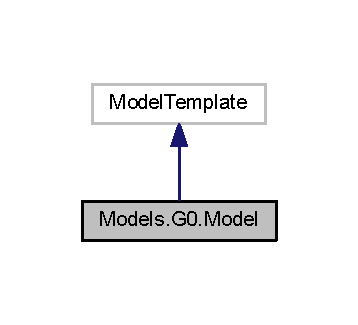
\includegraphics[width=172pt]{class_models_1_1_g0_1_1_model__inherit__graph}
\end{center}
\end{figure}


Collaboration diagram for Models.\-G0.\-Model\-:
\nopagebreak
\begin{figure}[H]
\begin{center}
\leavevmode
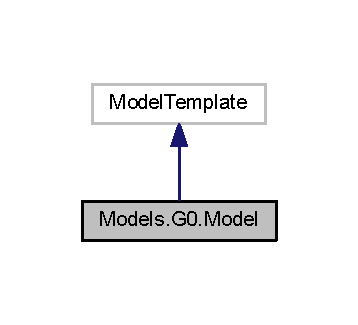
\includegraphics[width=172pt]{class_models_1_1_g0_1_1_model__coll__graph}
\end{center}
\end{figure}
\subsection*{Public Member Functions}
\begin{DoxyCompactItemize}
\item 
def \hyperlink{class_models_1_1_g0_1_1_model_a8f609350a16ab0dc5da6666b8b5602b3}{\-\_\-\-\_\-init\-\_\-\-\_\-}
\item 
def \hyperlink{class_models_1_1_g0_1_1_model_a60d4c047bc598240d4d5f8ef147c04d4}{calc\-\_\-b\-\_\-h\-\_\-vi}
\item 
def \hyperlink{class_models_1_1_g0_1_1_model_a42c7665f251f4821ef68fd5059d8f676}{calc\-\_\-b\-\_\-h}
\item 
def \hyperlink{class_models_1_1_g0_1_1_model_ae46d860ab0d25f883b93673e24fd7e06}{calc\-\_\-\-P\-\_\-h\-\_\-vi}
\item 
def \hyperlink{class_models_1_1_g0_1_1_model_aade1cb05e796c148ad4d1d9f1e7bdd37}{calc\-\_\-r\-\_\-vi}
\item 
def \hyperlink{class_models_1_1_g0_1_1_model_add79bd110862e1aa5db76907a6bbf163}{calc\-\_\-\-S\-\_\-vi}
\end{DoxyCompactItemize}


\subsection{Detailed Description}
\begin{DoxyVerb}Modelo\end{DoxyVerb}
 

\subsection{Constructor \& Destructor Documentation}
\hypertarget{class_models_1_1_g0_1_1_model_a8f609350a16ab0dc5da6666b8b5602b3}{\index{Models\-::\-G0\-::\-Model@{Models\-::\-G0\-::\-Model}!\-\_\-\-\_\-init\-\_\-\-\_\-@{\-\_\-\-\_\-init\-\_\-\-\_\-}}
\index{\-\_\-\-\_\-init\-\_\-\-\_\-@{\-\_\-\-\_\-init\-\_\-\-\_\-}!Models::G0::Model@{Models\-::\-G0\-::\-Model}}
\subsubsection[{\-\_\-\-\_\-init\-\_\-\-\_\-}]{\setlength{\rightskip}{0pt plus 5cm}def Models.\-G0.\-Model.\-\_\-\-\_\-init\-\_\-\-\_\- (
\begin{DoxyParamCaption}
\item[{}]{self, }
\item[{}]{model\-Name}
\end{DoxyParamCaption}
)}}\label{class_models_1_1_g0_1_1_model_a8f609350a16ab0dc5da6666b8b5602b3}


\subsection{Member Function Documentation}
\hypertarget{class_models_1_1_g0_1_1_model_a42c7665f251f4821ef68fd5059d8f676}{\index{Models\-::\-G0\-::\-Model@{Models\-::\-G0\-::\-Model}!calc\-\_\-b\-\_\-h@{calc\-\_\-b\-\_\-h}}
\index{calc\-\_\-b\-\_\-h@{calc\-\_\-b\-\_\-h}!Models::G0::Model@{Models\-::\-G0\-::\-Model}}
\subsubsection[{calc\-\_\-b\-\_\-h}]{\setlength{\rightskip}{0pt plus 5cm}def Models.\-G0.\-Model.\-calc\-\_\-b\-\_\-h (
\begin{DoxyParamCaption}
\item[{}]{self, }
\item[{}]{dm, }
\item[{}]{t}
\end{DoxyParamCaption}
)}}\label{class_models_1_1_g0_1_1_model_a42c7665f251f4821ef68fd5059d8f676}
\hypertarget{class_models_1_1_g0_1_1_model_a60d4c047bc598240d4d5f8ef147c04d4}{\index{Models\-::\-G0\-::\-Model@{Models\-::\-G0\-::\-Model}!calc\-\_\-b\-\_\-h\-\_\-vi@{calc\-\_\-b\-\_\-h\-\_\-vi}}
\index{calc\-\_\-b\-\_\-h\-\_\-vi@{calc\-\_\-b\-\_\-h\-\_\-vi}!Models::G0::Model@{Models\-::\-G0\-::\-Model}}
\subsubsection[{calc\-\_\-b\-\_\-h\-\_\-vi}]{\setlength{\rightskip}{0pt plus 5cm}def Models.\-G0.\-Model.\-calc\-\_\-b\-\_\-h\-\_\-vi (
\begin{DoxyParamCaption}
\item[{}]{self, }
\item[{}]{dm, }
\item[{}]{t}
\end{DoxyParamCaption}
)}}\label{class_models_1_1_g0_1_1_model_a60d4c047bc598240d4d5f8ef147c04d4}
\hypertarget{class_models_1_1_g0_1_1_model_ae46d860ab0d25f883b93673e24fd7e06}{\index{Models\-::\-G0\-::\-Model@{Models\-::\-G0\-::\-Model}!calc\-\_\-\-P\-\_\-h\-\_\-vi@{calc\-\_\-\-P\-\_\-h\-\_\-vi}}
\index{calc\-\_\-\-P\-\_\-h\-\_\-vi@{calc\-\_\-\-P\-\_\-h\-\_\-vi}!Models::G0::Model@{Models\-::\-G0\-::\-Model}}
\subsubsection[{calc\-\_\-\-P\-\_\-h\-\_\-vi}]{\setlength{\rightskip}{0pt plus 5cm}def Models.\-G0.\-Model.\-calc\-\_\-\-P\-\_\-h\-\_\-vi (
\begin{DoxyParamCaption}
\item[{}]{self, }
\item[{}]{dm, }
\item[{}]{t}
\end{DoxyParamCaption}
)}}\label{class_models_1_1_g0_1_1_model_ae46d860ab0d25f883b93673e24fd7e06}
\hypertarget{class_models_1_1_g0_1_1_model_aade1cb05e796c148ad4d1d9f1e7bdd37}{\index{Models\-::\-G0\-::\-Model@{Models\-::\-G0\-::\-Model}!calc\-\_\-r\-\_\-vi@{calc\-\_\-r\-\_\-vi}}
\index{calc\-\_\-r\-\_\-vi@{calc\-\_\-r\-\_\-vi}!Models::G0::Model@{Models\-::\-G0\-::\-Model}}
\subsubsection[{calc\-\_\-r\-\_\-vi}]{\setlength{\rightskip}{0pt plus 5cm}def Models.\-G0.\-Model.\-calc\-\_\-r\-\_\-vi (
\begin{DoxyParamCaption}
\item[{}]{self, }
\item[{}]{dm, }
\item[{}]{t}
\end{DoxyParamCaption}
)}}\label{class_models_1_1_g0_1_1_model_aade1cb05e796c148ad4d1d9f1e7bdd37}
\hypertarget{class_models_1_1_g0_1_1_model_add79bd110862e1aa5db76907a6bbf163}{\index{Models\-::\-G0\-::\-Model@{Models\-::\-G0\-::\-Model}!calc\-\_\-\-S\-\_\-vi@{calc\-\_\-\-S\-\_\-vi}}
\index{calc\-\_\-\-S\-\_\-vi@{calc\-\_\-\-S\-\_\-vi}!Models::G0::Model@{Models\-::\-G0\-::\-Model}}
\subsubsection[{calc\-\_\-\-S\-\_\-vi}]{\setlength{\rightskip}{0pt plus 5cm}def Models.\-G0.\-Model.\-calc\-\_\-\-S\-\_\-vi (
\begin{DoxyParamCaption}
\item[{}]{self, }
\item[{}]{dm, }
\item[{}]{t}
\end{DoxyParamCaption}
)}}\label{class_models_1_1_g0_1_1_model_add79bd110862e1aa5db76907a6bbf163}


The documentation for this class was generated from the following file\-:\begin{DoxyCompactItemize}
\item 
Models/\hyperlink{_g0_8py}{G0.\-py}\end{DoxyCompactItemize}

\hypertarget{class_models_1_1_gqs_rcon_1_1_model}{\section{Models.\-Gqs\-Rcon.\-Model Class Reference}
\label{class_models_1_1_gqs_rcon_1_1_model}\index{Models.\-Gqs\-Rcon.\-Model@{Models.\-Gqs\-Rcon.\-Model}}
}


Inheritance diagram for Models.\-Gqs\-Rcon.\-Model\-:
\nopagebreak
\begin{figure}[H]
\begin{center}
\leavevmode
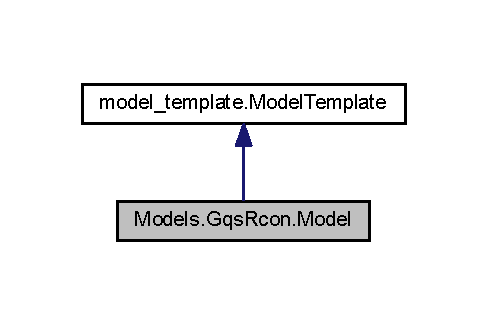
\includegraphics[width=234pt]{class_models_1_1_gqs_rcon_1_1_model__inherit__graph}
\end{center}
\end{figure}


Collaboration diagram for Models.\-Gqs\-Rcon.\-Model\-:
\nopagebreak
\begin{figure}[H]
\begin{center}
\leavevmode
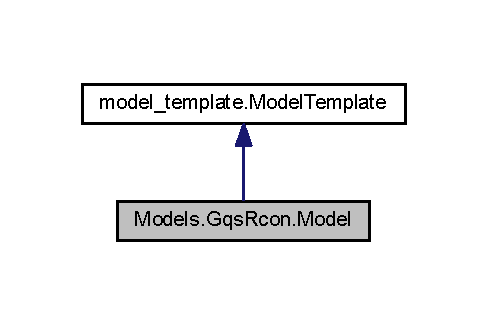
\includegraphics[width=234pt]{class_models_1_1_gqs_rcon_1_1_model__coll__graph}
\end{center}
\end{figure}
\subsection*{Public Member Functions}
\begin{DoxyCompactItemize}
\item 
def \hyperlink{class_models_1_1_gqs_rcon_1_1_model_a7c105d2b098c02a92d820b563b3f9626}{\-\_\-\-\_\-init\-\_\-\-\_\-}
\item 
def \hyperlink{class_models_1_1_gqs_rcon_1_1_model_a7c17483b4152aae30746e9020cc9b2a7}{calc\-\_\-b\-\_\-h\-\_\-vi}
\item 
def \hyperlink{class_models_1_1_gqs_rcon_1_1_model_acc67fde18afe6f23d15ee63365858643}{calc\-\_\-phi\-\_\-hvi}
\item 
def \hyperlink{class_models_1_1_gqs_rcon_1_1_model_a9e3520749c7bf68bfbd4285abf1ab9a5}{calc\-\_\-b\-\_\-h}
\item 
def \hyperlink{class_models_1_1_gqs_rcon_1_1_model_ae41680c4c2ab719168f233d2a75318bc}{calc\-\_\-\-P\-\_\-h\-\_\-vi}
\item 
def \hyperlink{class_models_1_1_gqs_rcon_1_1_model_a82100aed9f6ceec6608f48fa07b2de15}{calc\-\_\-r\-\_\-vi}
\item 
def \hyperlink{class_models_1_1_gqs_rcon_1_1_model_a1b18fbb828ecb04cd4b044f977bbe78c}{calc\-\_\-\-S\-\_\-vi}
\item 
def \hyperlink{class_models_1_1_gqs_rcon_1_1_model_a6480b364645c9906d56ac5448018ad27}{calc\-\_\-gamma\-\_\-vi}
\end{DoxyCompactItemize}
\subsection*{Additional Inherited Members}


\subsection{Detailed Description}
\begin{DoxyVerb}Modelo\end{DoxyVerb}
 

\subsection{Constructor \& Destructor Documentation}
\hypertarget{class_models_1_1_gqs_rcon_1_1_model_a7c105d2b098c02a92d820b563b3f9626}{\index{Models\-::\-Gqs\-Rcon\-::\-Model@{Models\-::\-Gqs\-Rcon\-::\-Model}!\-\_\-\-\_\-init\-\_\-\-\_\-@{\-\_\-\-\_\-init\-\_\-\-\_\-}}
\index{\-\_\-\-\_\-init\-\_\-\-\_\-@{\-\_\-\-\_\-init\-\_\-\-\_\-}!Models::GqsRcon::Model@{Models\-::\-Gqs\-Rcon\-::\-Model}}
\subsubsection[{\-\_\-\-\_\-init\-\_\-\-\_\-}]{\setlength{\rightskip}{0pt plus 5cm}def Models.\-Gqs\-Rcon.\-Model.\-\_\-\-\_\-init\-\_\-\-\_\- (
\begin{DoxyParamCaption}
\item[{}]{self, }
\item[{}]{model\-Name}
\end{DoxyParamCaption}
)}}\label{class_models_1_1_gqs_rcon_1_1_model_a7c105d2b098c02a92d820b563b3f9626}


\subsection{Member Function Documentation}
\hypertarget{class_models_1_1_gqs_rcon_1_1_model_a9e3520749c7bf68bfbd4285abf1ab9a5}{\index{Models\-::\-Gqs\-Rcon\-::\-Model@{Models\-::\-Gqs\-Rcon\-::\-Model}!calc\-\_\-b\-\_\-h@{calc\-\_\-b\-\_\-h}}
\index{calc\-\_\-b\-\_\-h@{calc\-\_\-b\-\_\-h}!Models::GqsRcon::Model@{Models\-::\-Gqs\-Rcon\-::\-Model}}
\subsubsection[{calc\-\_\-b\-\_\-h}]{\setlength{\rightskip}{0pt plus 5cm}def Models.\-Gqs\-Rcon.\-Model.\-calc\-\_\-b\-\_\-h (
\begin{DoxyParamCaption}
\item[{}]{self, }
\item[{}]{dm, }
\item[{}]{t}
\end{DoxyParamCaption}
)}}\label{class_models_1_1_gqs_rcon_1_1_model_a9e3520749c7bf68bfbd4285abf1ab9a5}
\hypertarget{class_models_1_1_gqs_rcon_1_1_model_a7c17483b4152aae30746e9020cc9b2a7}{\index{Models\-::\-Gqs\-Rcon\-::\-Model@{Models\-::\-Gqs\-Rcon\-::\-Model}!calc\-\_\-b\-\_\-h\-\_\-vi@{calc\-\_\-b\-\_\-h\-\_\-vi}}
\index{calc\-\_\-b\-\_\-h\-\_\-vi@{calc\-\_\-b\-\_\-h\-\_\-vi}!Models::GqsRcon::Model@{Models\-::\-Gqs\-Rcon\-::\-Model}}
\subsubsection[{calc\-\_\-b\-\_\-h\-\_\-vi}]{\setlength{\rightskip}{0pt plus 5cm}def Models.\-Gqs\-Rcon.\-Model.\-calc\-\_\-b\-\_\-h\-\_\-vi (
\begin{DoxyParamCaption}
\item[{}]{self, }
\item[{}]{dm, }
\item[{}]{t}
\end{DoxyParamCaption}
)}}\label{class_models_1_1_gqs_rcon_1_1_model_a7c17483b4152aae30746e9020cc9b2a7}
\hypertarget{class_models_1_1_gqs_rcon_1_1_model_a6480b364645c9906d56ac5448018ad27}{\index{Models\-::\-Gqs\-Rcon\-::\-Model@{Models\-::\-Gqs\-Rcon\-::\-Model}!calc\-\_\-gamma\-\_\-vi@{calc\-\_\-gamma\-\_\-vi}}
\index{calc\-\_\-gamma\-\_\-vi@{calc\-\_\-gamma\-\_\-vi}!Models::GqsRcon::Model@{Models\-::\-Gqs\-Rcon\-::\-Model}}
\subsubsection[{calc\-\_\-gamma\-\_\-vi}]{\setlength{\rightskip}{0pt plus 5cm}def Models.\-Gqs\-Rcon.\-Model.\-calc\-\_\-gamma\-\_\-vi (
\begin{DoxyParamCaption}
\item[{}]{self, }
\item[{}]{dm, }
\item[{}]{t}
\end{DoxyParamCaption}
)}}\label{class_models_1_1_gqs_rcon_1_1_model_a6480b364645c9906d56ac5448018ad27}
\hypertarget{class_models_1_1_gqs_rcon_1_1_model_ae41680c4c2ab719168f233d2a75318bc}{\index{Models\-::\-Gqs\-Rcon\-::\-Model@{Models\-::\-Gqs\-Rcon\-::\-Model}!calc\-\_\-\-P\-\_\-h\-\_\-vi@{calc\-\_\-\-P\-\_\-h\-\_\-vi}}
\index{calc\-\_\-\-P\-\_\-h\-\_\-vi@{calc\-\_\-\-P\-\_\-h\-\_\-vi}!Models::GqsRcon::Model@{Models\-::\-Gqs\-Rcon\-::\-Model}}
\subsubsection[{calc\-\_\-\-P\-\_\-h\-\_\-vi}]{\setlength{\rightskip}{0pt plus 5cm}def Models.\-Gqs\-Rcon.\-Model.\-calc\-\_\-\-P\-\_\-h\-\_\-vi (
\begin{DoxyParamCaption}
\item[{}]{self, }
\item[{}]{dm, }
\item[{}]{t}
\end{DoxyParamCaption}
)}}\label{class_models_1_1_gqs_rcon_1_1_model_ae41680c4c2ab719168f233d2a75318bc}
\hypertarget{class_models_1_1_gqs_rcon_1_1_model_acc67fde18afe6f23d15ee63365858643}{\index{Models\-::\-Gqs\-Rcon\-::\-Model@{Models\-::\-Gqs\-Rcon\-::\-Model}!calc\-\_\-phi\-\_\-hvi@{calc\-\_\-phi\-\_\-hvi}}
\index{calc\-\_\-phi\-\_\-hvi@{calc\-\_\-phi\-\_\-hvi}!Models::GqsRcon::Model@{Models\-::\-Gqs\-Rcon\-::\-Model}}
\subsubsection[{calc\-\_\-phi\-\_\-hvi}]{\setlength{\rightskip}{0pt plus 5cm}def Models.\-Gqs\-Rcon.\-Model.\-calc\-\_\-phi\-\_\-hvi (
\begin{DoxyParamCaption}
\item[{}]{self, }
\item[{}]{dm, }
\item[{}]{t}
\end{DoxyParamCaption}
)}}\label{class_models_1_1_gqs_rcon_1_1_model_acc67fde18afe6f23d15ee63365858643}
\hypertarget{class_models_1_1_gqs_rcon_1_1_model_a82100aed9f6ceec6608f48fa07b2de15}{\index{Models\-::\-Gqs\-Rcon\-::\-Model@{Models\-::\-Gqs\-Rcon\-::\-Model}!calc\-\_\-r\-\_\-vi@{calc\-\_\-r\-\_\-vi}}
\index{calc\-\_\-r\-\_\-vi@{calc\-\_\-r\-\_\-vi}!Models::GqsRcon::Model@{Models\-::\-Gqs\-Rcon\-::\-Model}}
\subsubsection[{calc\-\_\-r\-\_\-vi}]{\setlength{\rightskip}{0pt plus 5cm}def Models.\-Gqs\-Rcon.\-Model.\-calc\-\_\-r\-\_\-vi (
\begin{DoxyParamCaption}
\item[{}]{self, }
\item[{}]{dm, }
\item[{}]{t}
\end{DoxyParamCaption}
)}}\label{class_models_1_1_gqs_rcon_1_1_model_a82100aed9f6ceec6608f48fa07b2de15}
\hypertarget{class_models_1_1_gqs_rcon_1_1_model_a1b18fbb828ecb04cd4b044f977bbe78c}{\index{Models\-::\-Gqs\-Rcon\-::\-Model@{Models\-::\-Gqs\-Rcon\-::\-Model}!calc\-\_\-\-S\-\_\-vi@{calc\-\_\-\-S\-\_\-vi}}
\index{calc\-\_\-\-S\-\_\-vi@{calc\-\_\-\-S\-\_\-vi}!Models::GqsRcon::Model@{Models\-::\-Gqs\-Rcon\-::\-Model}}
\subsubsection[{calc\-\_\-\-S\-\_\-vi}]{\setlength{\rightskip}{0pt plus 5cm}def Models.\-Gqs\-Rcon.\-Model.\-calc\-\_\-\-S\-\_\-vi (
\begin{DoxyParamCaption}
\item[{}]{self, }
\item[{}]{dm, }
\item[{}]{t}
\end{DoxyParamCaption}
)}}\label{class_models_1_1_gqs_rcon_1_1_model_a1b18fbb828ecb04cd4b044f977bbe78c}


The documentation for this class was generated from the following file\-:\begin{DoxyCompactItemize}
\item 
Models/\hyperlink{_gqs_rcon_8py}{Gqs\-Rcon.\-py}\end{DoxyCompactItemize}

\hypertarget{classmodel__template_1_1_model_template}{\section{model\-\_\-template.\-Model\-Template Class Reference}
\label{classmodel__template_1_1_model_template}\index{model\-\_\-template.\-Model\-Template@{model\-\_\-template.\-Model\-Template}}
}


Inheritance diagram for model\-\_\-template.\-Model\-Template\-:
\nopagebreak
\begin{figure}[H]
\begin{center}
\leavevmode
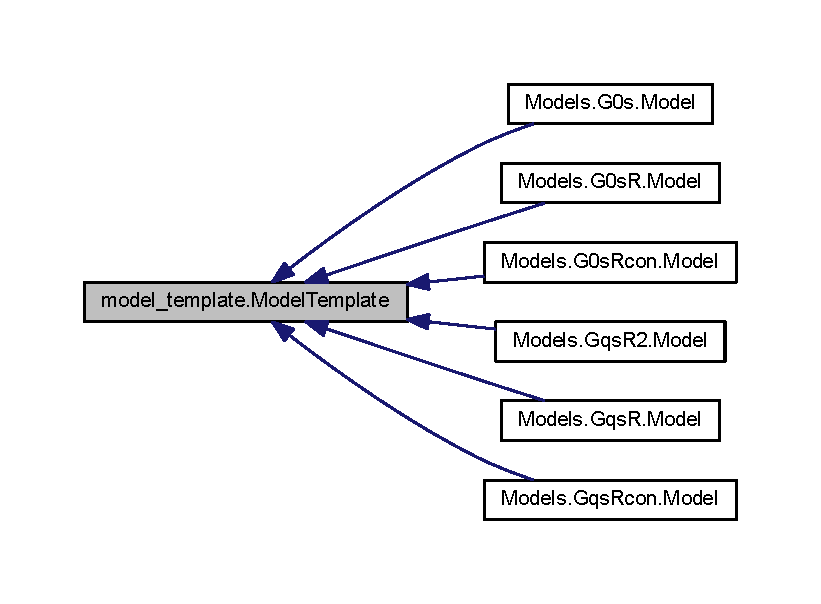
\includegraphics[width=350pt]{classmodel__template_1_1_model_template__inherit__graph}
\end{center}
\end{figure}
\subsection*{Public Member Functions}
\begin{DoxyCompactItemize}
\item 
def \hyperlink{classmodel__template_1_1_model_template_a22197c6b1c038b67b9f414b2a0b12846}{\-\_\-\-\_\-init\-\_\-\-\_\-}
\item 
def \hyperlink{classmodel__template_1_1_model_template_af0d165e3670fa2ab8dc95fccbd1000fc}{ejecutar}
\item 
def \hyperlink{classmodel__template_1_1_model_template_a9727f5ca1d701411213cc94c9ce03794}{calc\-\_\-delta}
\item 
def \hyperlink{classmodel__template_1_1_model_template_a99a7f880441811cf7b09780bf099115f}{calc\-\_\-b\-\_\-h}
\item 
def \hyperlink{classmodel__template_1_1_model_template_a9f8c5a5dc9e9a2398b58f72a78fc6f2a}{calc\-\_\-\-P\-\_\-h\-\_\-vi}
\item 
def \hyperlink{classmodel__template_1_1_model_template_af83077979e5346923e200bbafbfbeae4}{calc\-\_\-r\-\_\-vi}
\item 
def \hyperlink{classmodel__template_1_1_model_template_aa32093145d0c97c2b57c19c050fe45ed}{calc\-\_\-\-S\-\_\-vi}
\item 
def \hyperlink{classmodel__template_1_1_model_template_ab811af1260ed4508b9a7b9add11ddaa7}{calc\-\_\-b\-\_\-h\-\_\-vi}
\item 
def \hyperlink{classmodel__template_1_1_model_template_adc23f1d97101b711175e59567f42d31e}{calc\-\_\-gamma\-\_\-vi}
\item 
def \hyperlink{classmodel__template_1_1_model_template_af619b3107d5ec929898af992d0f808e8}{calc\-\_\-phi\-\_\-hvi}
\item 
def \hyperlink{classmodel__template_1_1_model_template_a6a38f083f47055d4a133efdb0172276d}{calc\-\_\-\-H\-\_\-h\-\_\-vi}
\item 
def \hyperlink{classmodel__template_1_1_model_template_a09ce6d25691672785a5ea7c980f0759d}{calc\-\_\-\-I\-\_\-h\-\_\-vi}
\item 
def \hyperlink{classmodel__template_1_1_model_template_a2bd2a69420be014cdf22d3656027ea29}{calc\-\_\-\-B\-\_\-h\-\_\-vi}
\item 
def \hyperlink{classmodel__template_1_1_model_template_a4fae6780c272da5c8c01e9fde800bb01}{calc\-\_\-\-I2}
\item 
def \hyperlink{classmodel__template_1_1_model_template_a304db21d5d560062f31e5c2493406f1c}{calc\-\_\-avg\-Z\-\_\-vi}
\item 
def \hyperlink{classmodel__template_1_1_model_template_a2f35480a0987ceacd1737c12f8398bb0}{imprimir\-\_\-iter}
\end{DoxyCompactItemize}
\subsection*{Public Attributes}
\begin{DoxyCompactItemize}
\item 
\hyperlink{classmodel__template_1_1_model_template_af42a05f8a957908da3221e8162f18951}{N\-O\-M\-B\-R\-E\-\_\-\-M\-O\-D\-E\-L\-O}
\item 
\hyperlink{classmodel__template_1_1_model_template_adfeedfd46f8495de3949aaf6353c8a74}{cnt}
\item 
\hyperlink{classmodel__template_1_1_model_template_a59aa8b91217b8ec30ec1c01faef3af80}{curr}
\item 
\hyperlink{classmodel__template_1_1_model_template_aa175ad27a71d7ed36174a51cf10cf07f}{delta}
\item 
\hyperlink{classmodel__template_1_1_model_template_acc16ac1b6b215e780256326d5bbe0355}{old}
\end{DoxyCompactItemize}


\subsection{Detailed Description}
\begin{DoxyVerb}Modelo\end{DoxyVerb}
 

\subsection{Constructor \& Destructor Documentation}
\hypertarget{classmodel__template_1_1_model_template_a22197c6b1c038b67b9f414b2a0b12846}{\index{model\-\_\-template\-::\-Model\-Template@{model\-\_\-template\-::\-Model\-Template}!\-\_\-\-\_\-init\-\_\-\-\_\-@{\-\_\-\-\_\-init\-\_\-\-\_\-}}
\index{\-\_\-\-\_\-init\-\_\-\-\_\-@{\-\_\-\-\_\-init\-\_\-\-\_\-}!model_template::ModelTemplate@{model\-\_\-template\-::\-Model\-Template}}
\subsubsection[{\-\_\-\-\_\-init\-\_\-\-\_\-}]{\setlength{\rightskip}{0pt plus 5cm}def model\-\_\-template.\-Model\-Template.\-\_\-\-\_\-init\-\_\-\-\_\- (
\begin{DoxyParamCaption}
\item[{}]{self, }
\item[{}]{N\-O\-M\-B\-R\-E\-\_\-\-M\-O\-D\-E\-L\-O}
\end{DoxyParamCaption}
)}}\label{classmodel__template_1_1_model_template_a22197c6b1c038b67b9f414b2a0b12846}


\subsection{Member Function Documentation}
\hypertarget{classmodel__template_1_1_model_template_a304db21d5d560062f31e5c2493406f1c}{\index{model\-\_\-template\-::\-Model\-Template@{model\-\_\-template\-::\-Model\-Template}!calc\-\_\-avg\-Z\-\_\-vi@{calc\-\_\-avg\-Z\-\_\-vi}}
\index{calc\-\_\-avg\-Z\-\_\-vi@{calc\-\_\-avg\-Z\-\_\-vi}!model_template::ModelTemplate@{model\-\_\-template\-::\-Model\-Template}}
\subsubsection[{calc\-\_\-avg\-Z\-\_\-vi}]{\setlength{\rightskip}{0pt plus 5cm}def model\-\_\-template.\-Model\-Template.\-calc\-\_\-avg\-Z\-\_\-vi (
\begin{DoxyParamCaption}
\item[{}]{self, }
\item[{}]{dm}
\end{DoxyParamCaption}
)}}\label{classmodel__template_1_1_model_template_a304db21d5d560062f31e5c2493406f1c}
\hypertarget{classmodel__template_1_1_model_template_a99a7f880441811cf7b09780bf099115f}{\index{model\-\_\-template\-::\-Model\-Template@{model\-\_\-template\-::\-Model\-Template}!calc\-\_\-b\-\_\-h@{calc\-\_\-b\-\_\-h}}
\index{calc\-\_\-b\-\_\-h@{calc\-\_\-b\-\_\-h}!model_template::ModelTemplate@{model\-\_\-template\-::\-Model\-Template}}
\subsubsection[{calc\-\_\-b\-\_\-h}]{\setlength{\rightskip}{0pt plus 5cm}def model\-\_\-template.\-Model\-Template.\-calc\-\_\-b\-\_\-h (
\begin{DoxyParamCaption}
\item[{}]{self, }
\item[{}]{dm, }
\item[{}]{t}
\end{DoxyParamCaption}
)}}\label{classmodel__template_1_1_model_template_a99a7f880441811cf7b09780bf099115f}
\hypertarget{classmodel__template_1_1_model_template_ab811af1260ed4508b9a7b9add11ddaa7}{\index{model\-\_\-template\-::\-Model\-Template@{model\-\_\-template\-::\-Model\-Template}!calc\-\_\-b\-\_\-h\-\_\-vi@{calc\-\_\-b\-\_\-h\-\_\-vi}}
\index{calc\-\_\-b\-\_\-h\-\_\-vi@{calc\-\_\-b\-\_\-h\-\_\-vi}!model_template::ModelTemplate@{model\-\_\-template\-::\-Model\-Template}}
\subsubsection[{calc\-\_\-b\-\_\-h\-\_\-vi}]{\setlength{\rightskip}{0pt plus 5cm}def model\-\_\-template.\-Model\-Template.\-calc\-\_\-b\-\_\-h\-\_\-vi (
\begin{DoxyParamCaption}
\item[{}]{self, }
\item[{}]{dm}
\end{DoxyParamCaption}
)}}\label{classmodel__template_1_1_model_template_ab811af1260ed4508b9a7b9add11ddaa7}
\hypertarget{classmodel__template_1_1_model_template_a2bd2a69420be014cdf22d3656027ea29}{\index{model\-\_\-template\-::\-Model\-Template@{model\-\_\-template\-::\-Model\-Template}!calc\-\_\-\-B\-\_\-h\-\_\-vi@{calc\-\_\-\-B\-\_\-h\-\_\-vi}}
\index{calc\-\_\-\-B\-\_\-h\-\_\-vi@{calc\-\_\-\-B\-\_\-h\-\_\-vi}!model_template::ModelTemplate@{model\-\_\-template\-::\-Model\-Template}}
\subsubsection[{calc\-\_\-\-B\-\_\-h\-\_\-vi}]{\setlength{\rightskip}{0pt plus 5cm}def model\-\_\-template.\-Model\-Template.\-calc\-\_\-\-B\-\_\-h\-\_\-vi (
\begin{DoxyParamCaption}
\item[{}]{self}
\end{DoxyParamCaption}
)}}\label{classmodel__template_1_1_model_template_a2bd2a69420be014cdf22d3656027ea29}
\hypertarget{classmodel__template_1_1_model_template_a9727f5ca1d701411213cc94c9ce03794}{\index{model\-\_\-template\-::\-Model\-Template@{model\-\_\-template\-::\-Model\-Template}!calc\-\_\-delta@{calc\-\_\-delta}}
\index{calc\-\_\-delta@{calc\-\_\-delta}!model_template::ModelTemplate@{model\-\_\-template\-::\-Model\-Template}}
\subsubsection[{calc\-\_\-delta}]{\setlength{\rightskip}{0pt plus 5cm}def model\-\_\-template.\-Model\-Template.\-calc\-\_\-delta (
\begin{DoxyParamCaption}
\item[{}]{self}
\end{DoxyParamCaption}
)}}\label{classmodel__template_1_1_model_template_a9727f5ca1d701411213cc94c9ce03794}
\hypertarget{classmodel__template_1_1_model_template_adc23f1d97101b711175e59567f42d31e}{\index{model\-\_\-template\-::\-Model\-Template@{model\-\_\-template\-::\-Model\-Template}!calc\-\_\-gamma\-\_\-vi@{calc\-\_\-gamma\-\_\-vi}}
\index{calc\-\_\-gamma\-\_\-vi@{calc\-\_\-gamma\-\_\-vi}!model_template::ModelTemplate@{model\-\_\-template\-::\-Model\-Template}}
\subsubsection[{calc\-\_\-gamma\-\_\-vi}]{\setlength{\rightskip}{0pt plus 5cm}def model\-\_\-template.\-Model\-Template.\-calc\-\_\-gamma\-\_\-vi (
\begin{DoxyParamCaption}
\item[{}]{self, }
\item[{}]{dm, }
\item[{}]{t}
\end{DoxyParamCaption}
)}}\label{classmodel__template_1_1_model_template_adc23f1d97101b711175e59567f42d31e}
\hypertarget{classmodel__template_1_1_model_template_a6a38f083f47055d4a133efdb0172276d}{\index{model\-\_\-template\-::\-Model\-Template@{model\-\_\-template\-::\-Model\-Template}!calc\-\_\-\-H\-\_\-h\-\_\-vi@{calc\-\_\-\-H\-\_\-h\-\_\-vi}}
\index{calc\-\_\-\-H\-\_\-h\-\_\-vi@{calc\-\_\-\-H\-\_\-h\-\_\-vi}!model_template::ModelTemplate@{model\-\_\-template\-::\-Model\-Template}}
\subsubsection[{calc\-\_\-\-H\-\_\-h\-\_\-vi}]{\setlength{\rightskip}{0pt plus 5cm}def model\-\_\-template.\-Model\-Template.\-calc\-\_\-\-H\-\_\-h\-\_\-vi (
\begin{DoxyParamCaption}
\item[{}]{self}
\end{DoxyParamCaption}
)}}\label{classmodel__template_1_1_model_template_a6a38f083f47055d4a133efdb0172276d}
\hypertarget{classmodel__template_1_1_model_template_a4fae6780c272da5c8c01e9fde800bb01}{\index{model\-\_\-template\-::\-Model\-Template@{model\-\_\-template\-::\-Model\-Template}!calc\-\_\-\-I2@{calc\-\_\-\-I2}}
\index{calc\-\_\-\-I2@{calc\-\_\-\-I2}!model_template::ModelTemplate@{model\-\_\-template\-::\-Model\-Template}}
\subsubsection[{calc\-\_\-\-I2}]{\setlength{\rightskip}{0pt plus 5cm}def model\-\_\-template.\-Model\-Template.\-calc\-\_\-\-I2 (
\begin{DoxyParamCaption}
\item[{}]{self, }
\item[{}]{dm}
\end{DoxyParamCaption}
)}}\label{classmodel__template_1_1_model_template_a4fae6780c272da5c8c01e9fde800bb01}
\hypertarget{classmodel__template_1_1_model_template_a09ce6d25691672785a5ea7c980f0759d}{\index{model\-\_\-template\-::\-Model\-Template@{model\-\_\-template\-::\-Model\-Template}!calc\-\_\-\-I\-\_\-h\-\_\-vi@{calc\-\_\-\-I\-\_\-h\-\_\-vi}}
\index{calc\-\_\-\-I\-\_\-h\-\_\-vi@{calc\-\_\-\-I\-\_\-h\-\_\-vi}!model_template::ModelTemplate@{model\-\_\-template\-::\-Model\-Template}}
\subsubsection[{calc\-\_\-\-I\-\_\-h\-\_\-vi}]{\setlength{\rightskip}{0pt plus 5cm}def model\-\_\-template.\-Model\-Template.\-calc\-\_\-\-I\-\_\-h\-\_\-vi (
\begin{DoxyParamCaption}
\item[{}]{self}
\end{DoxyParamCaption}
)}}\label{classmodel__template_1_1_model_template_a09ce6d25691672785a5ea7c980f0759d}
\hypertarget{classmodel__template_1_1_model_template_a9f8c5a5dc9e9a2398b58f72a78fc6f2a}{\index{model\-\_\-template\-::\-Model\-Template@{model\-\_\-template\-::\-Model\-Template}!calc\-\_\-\-P\-\_\-h\-\_\-vi@{calc\-\_\-\-P\-\_\-h\-\_\-vi}}
\index{calc\-\_\-\-P\-\_\-h\-\_\-vi@{calc\-\_\-\-P\-\_\-h\-\_\-vi}!model_template::ModelTemplate@{model\-\_\-template\-::\-Model\-Template}}
\subsubsection[{calc\-\_\-\-P\-\_\-h\-\_\-vi}]{\setlength{\rightskip}{0pt plus 5cm}def model\-\_\-template.\-Model\-Template.\-calc\-\_\-\-P\-\_\-h\-\_\-vi (
\begin{DoxyParamCaption}
\item[{}]{self, }
\item[{}]{dm, }
\item[{}]{t}
\end{DoxyParamCaption}
)}}\label{classmodel__template_1_1_model_template_a9f8c5a5dc9e9a2398b58f72a78fc6f2a}
\hypertarget{classmodel__template_1_1_model_template_af619b3107d5ec929898af992d0f808e8}{\index{model\-\_\-template\-::\-Model\-Template@{model\-\_\-template\-::\-Model\-Template}!calc\-\_\-phi\-\_\-hvi@{calc\-\_\-phi\-\_\-hvi}}
\index{calc\-\_\-phi\-\_\-hvi@{calc\-\_\-phi\-\_\-hvi}!model_template::ModelTemplate@{model\-\_\-template\-::\-Model\-Template}}
\subsubsection[{calc\-\_\-phi\-\_\-hvi}]{\setlength{\rightskip}{0pt plus 5cm}def model\-\_\-template.\-Model\-Template.\-calc\-\_\-phi\-\_\-hvi (
\begin{DoxyParamCaption}
\item[{}]{self, }
\item[{}]{dm, }
\item[{}]{t}
\end{DoxyParamCaption}
)}}\label{classmodel__template_1_1_model_template_af619b3107d5ec929898af992d0f808e8}
\hypertarget{classmodel__template_1_1_model_template_af83077979e5346923e200bbafbfbeae4}{\index{model\-\_\-template\-::\-Model\-Template@{model\-\_\-template\-::\-Model\-Template}!calc\-\_\-r\-\_\-vi@{calc\-\_\-r\-\_\-vi}}
\index{calc\-\_\-r\-\_\-vi@{calc\-\_\-r\-\_\-vi}!model_template::ModelTemplate@{model\-\_\-template\-::\-Model\-Template}}
\subsubsection[{calc\-\_\-r\-\_\-vi}]{\setlength{\rightskip}{0pt plus 5cm}def model\-\_\-template.\-Model\-Template.\-calc\-\_\-r\-\_\-vi (
\begin{DoxyParamCaption}
\item[{}]{self, }
\item[{}]{dm, }
\item[{}]{t}
\end{DoxyParamCaption}
)}}\label{classmodel__template_1_1_model_template_af83077979e5346923e200bbafbfbeae4}
\hypertarget{classmodel__template_1_1_model_template_aa32093145d0c97c2b57c19c050fe45ed}{\index{model\-\_\-template\-::\-Model\-Template@{model\-\_\-template\-::\-Model\-Template}!calc\-\_\-\-S\-\_\-vi@{calc\-\_\-\-S\-\_\-vi}}
\index{calc\-\_\-\-S\-\_\-vi@{calc\-\_\-\-S\-\_\-vi}!model_template::ModelTemplate@{model\-\_\-template\-::\-Model\-Template}}
\subsubsection[{calc\-\_\-\-S\-\_\-vi}]{\setlength{\rightskip}{0pt plus 5cm}def model\-\_\-template.\-Model\-Template.\-calc\-\_\-\-S\-\_\-vi (
\begin{DoxyParamCaption}
\item[{}]{self, }
\item[{}]{dm, }
\item[{}]{t}
\end{DoxyParamCaption}
)}}\label{classmodel__template_1_1_model_template_aa32093145d0c97c2b57c19c050fe45ed}
\hypertarget{classmodel__template_1_1_model_template_af0d165e3670fa2ab8dc95fccbd1000fc}{\index{model\-\_\-template\-::\-Model\-Template@{model\-\_\-template\-::\-Model\-Template}!ejecutar@{ejecutar}}
\index{ejecutar@{ejecutar}!model_template::ModelTemplate@{model\-\_\-template\-::\-Model\-Template}}
\subsubsection[{ejecutar}]{\setlength{\rightskip}{0pt plus 5cm}def model\-\_\-template.\-Model\-Template.\-ejecutar (
\begin{DoxyParamCaption}
\item[{}]{self, }
\item[{}]{dm, }
\item[{}]{t, }
\item[{}]{curr\-Output\-Folder\-Path = {\ttfamily \char`\"{}\char`\"{}}}
\end{DoxyParamCaption}
)}}\label{classmodel__template_1_1_model_template_af0d165e3670fa2ab8dc95fccbd1000fc}
\hypertarget{classmodel__template_1_1_model_template_a2f35480a0987ceacd1737c12f8398bb0}{\index{model\-\_\-template\-::\-Model\-Template@{model\-\_\-template\-::\-Model\-Template}!imprimir\-\_\-iter@{imprimir\-\_\-iter}}
\index{imprimir\-\_\-iter@{imprimir\-\_\-iter}!model_template::ModelTemplate@{model\-\_\-template\-::\-Model\-Template}}
\subsubsection[{imprimir\-\_\-iter}]{\setlength{\rightskip}{0pt plus 5cm}def model\-\_\-template.\-Model\-Template.\-imprimir\-\_\-iter (
\begin{DoxyParamCaption}
\item[{}]{self, }
\item[{}]{dm, }
\item[{}]{ff}
\end{DoxyParamCaption}
)}}\label{classmodel__template_1_1_model_template_a2f35480a0987ceacd1737c12f8398bb0}


\subsection{Member Data Documentation}
\hypertarget{classmodel__template_1_1_model_template_adfeedfd46f8495de3949aaf6353c8a74}{\index{model\-\_\-template\-::\-Model\-Template@{model\-\_\-template\-::\-Model\-Template}!cnt@{cnt}}
\index{cnt@{cnt}!model_template::ModelTemplate@{model\-\_\-template\-::\-Model\-Template}}
\subsubsection[{cnt}]{\setlength{\rightskip}{0pt plus 5cm}model\-\_\-template.\-Model\-Template.\-cnt}}\label{classmodel__template_1_1_model_template_adfeedfd46f8495de3949aaf6353c8a74}
\hypertarget{classmodel__template_1_1_model_template_a59aa8b91217b8ec30ec1c01faef3af80}{\index{model\-\_\-template\-::\-Model\-Template@{model\-\_\-template\-::\-Model\-Template}!curr@{curr}}
\index{curr@{curr}!model_template::ModelTemplate@{model\-\_\-template\-::\-Model\-Template}}
\subsubsection[{curr}]{\setlength{\rightskip}{0pt plus 5cm}model\-\_\-template.\-Model\-Template.\-curr}}\label{classmodel__template_1_1_model_template_a59aa8b91217b8ec30ec1c01faef3af80}
\hypertarget{classmodel__template_1_1_model_template_aa175ad27a71d7ed36174a51cf10cf07f}{\index{model\-\_\-template\-::\-Model\-Template@{model\-\_\-template\-::\-Model\-Template}!delta@{delta}}
\index{delta@{delta}!model_template::ModelTemplate@{model\-\_\-template\-::\-Model\-Template}}
\subsubsection[{delta}]{\setlength{\rightskip}{0pt plus 5cm}model\-\_\-template.\-Model\-Template.\-delta}}\label{classmodel__template_1_1_model_template_aa175ad27a71d7ed36174a51cf10cf07f}
\hypertarget{classmodel__template_1_1_model_template_af42a05f8a957908da3221e8162f18951}{\index{model\-\_\-template\-::\-Model\-Template@{model\-\_\-template\-::\-Model\-Template}!N\-O\-M\-B\-R\-E\-\_\-\-M\-O\-D\-E\-L\-O@{N\-O\-M\-B\-R\-E\-\_\-\-M\-O\-D\-E\-L\-O}}
\index{N\-O\-M\-B\-R\-E\-\_\-\-M\-O\-D\-E\-L\-O@{N\-O\-M\-B\-R\-E\-\_\-\-M\-O\-D\-E\-L\-O}!model_template::ModelTemplate@{model\-\_\-template\-::\-Model\-Template}}
\subsubsection[{N\-O\-M\-B\-R\-E\-\_\-\-M\-O\-D\-E\-L\-O}]{\setlength{\rightskip}{0pt plus 5cm}model\-\_\-template.\-Model\-Template.\-N\-O\-M\-B\-R\-E\-\_\-\-M\-O\-D\-E\-L\-O}}\label{classmodel__template_1_1_model_template_af42a05f8a957908da3221e8162f18951}
\hypertarget{classmodel__template_1_1_model_template_acc16ac1b6b215e780256326d5bbe0355}{\index{model\-\_\-template\-::\-Model\-Template@{model\-\_\-template\-::\-Model\-Template}!old@{old}}
\index{old@{old}!model_template::ModelTemplate@{model\-\_\-template\-::\-Model\-Template}}
\subsubsection[{old}]{\setlength{\rightskip}{0pt plus 5cm}model\-\_\-template.\-Model\-Template.\-old}}\label{classmodel__template_1_1_model_template_acc16ac1b6b215e780256326d5bbe0355}


The documentation for this class was generated from the following file\-:\begin{DoxyCompactItemize}
\item 
\hyperlink{model__template_8py}{model\-\_\-template.\-py}\end{DoxyCompactItemize}

\chapter{File Documentation}
\hypertarget{custom__file__reader_8py}{\section{custom\-\_\-file\-\_\-reader.\-py File Reference}
\label{custom__file__reader_8py}\index{custom\-\_\-file\-\_\-reader.\-py@{custom\-\_\-file\-\_\-reader.\-py}}
}
\subsection*{Classes}
\begin{DoxyCompactItemize}
\item 
class \hyperlink{classcustom__file__reader_1_1_custom_file_reader}{custom\-\_\-file\-\_\-reader.\-Custom\-File\-Reader}
\end{DoxyCompactItemize}
\subsection*{Namespaces}
\begin{DoxyCompactItemize}
\item 
namespace \hyperlink{namespacecustom__file__reader}{custom\-\_\-file\-\_\-reader}
\end{DoxyCompactItemize}

\hypertarget{data__manager_8py}{\section{data\-\_\-manager.\-py File Reference}
\label{data__manager_8py}\index{data\-\_\-manager.\-py@{data\-\_\-manager.\-py}}
}
\subsection*{Classes}
\begin{DoxyCompactItemize}
\item 
class \hyperlink{classdata__manager_1_1_data_manager}{data\-\_\-manager.\-Data\-Manager}
\end{DoxyCompactItemize}
\subsection*{Namespaces}
\begin{DoxyCompactItemize}
\item 
namespace \hyperlink{namespacedata__manager}{data\-\_\-manager}
\end{DoxyCompactItemize}

\hypertarget{data__plot_8py}{\section{data\-\_\-plot.\-py File Reference}
\label{data__plot_8py}\index{data\-\_\-plot.\-py@{data\-\_\-plot.\-py}}
}
\subsection*{Namespaces}
\begin{DoxyCompactItemize}
\item 
namespace \hyperlink{namespacedata__plot}{data\-\_\-plot}
\end{DoxyCompactItemize}
\subsection*{Functions}
\begin{DoxyCompactItemize}
\item 
def \hyperlink{namespacedata__plot_ae5595ad2b553b397c5737236e68b5ac0}{data\-\_\-plot.\-plot2}
\item 
def \hyperlink{namespacedata__plot_ab1e2fbbf96e3102b5af9834fd2a9afe6}{data\-\_\-plot.\-autolabel}
\item 
def \hyperlink{namespacedata__plot_aa83ee5efa7f8257501db891963e6cd42}{data\-\_\-plot.\-pastel}
\item 
def \hyperlink{namespacedata__plot_a561eca3a1a19ba1dd334d4ebabbb62d8}{data\-\_\-plot.\-get\-\_\-colours}
\end{DoxyCompactItemize}
\subsection*{Variables}
\begin{DoxyCompactItemize}
\item 
tuple \hyperlink{namespacedata__plot_ab643ddfd537318e86ad280cd29d6c741}{data\-\_\-plot.\-fload} = open(sys.\-argv\mbox{[}1\mbox{]}+\char`\"{}.dat\char`\"{},'r')
\item 
tuple \hyperlink{namespacedata__plot_a059a797dd0a7e613b2712934dc64140a}{data\-\_\-plot.\-dm} = pickle.\-load(fload)
\end{DoxyCompactItemize}

\hypertarget{data__struct_8py}{\section{data\-\_\-struct.\-py File Reference}
\label{data__struct_8py}\index{data\-\_\-struct.\-py@{data\-\_\-struct.\-py}}
}
\subsection*{Classes}
\begin{DoxyCompactItemize}
\item 
class \hyperlink{classdata__struct_1_1_data_struct}{data\-\_\-struct.\-Data\-Struct}
\end{DoxyCompactItemize}
\subsection*{Namespaces}
\begin{DoxyCompactItemize}
\item 
namespace \hyperlink{namespacedata__struct}{data\-\_\-struct}
\end{DoxyCompactItemize}

\hypertarget{model__template_8py}{\section{model\-\_\-template.\-py File Reference}
\label{model__template_8py}\index{model\-\_\-template.\-py@{model\-\_\-template.\-py}}
}
\subsection*{Classes}
\begin{DoxyCompactItemize}
\item 
class \hyperlink{classmodel__template_1_1_model_template}{model\-\_\-template.\-Model\-Template}
\end{DoxyCompactItemize}
\subsection*{Namespaces}
\begin{DoxyCompactItemize}
\item 
namespace \hyperlink{namespacemodel__template}{model\-\_\-template}
\end{DoxyCompactItemize}

\hypertarget{____init_____8py}{\section{Models/\-\_\-\-\_\-init\-\_\-\-\_\-.py File Reference}
\label{____init_____8py}\index{Models/\-\_\-\-\_\-init\-\_\-\-\_\-.\-py@{Models/\-\_\-\-\_\-init\-\_\-\-\_\-.\-py}}
}
\subsection*{Namespaces}
\begin{DoxyCompactItemize}
\item 
namespace \hyperlink{namespace_models}{Models}
\end{DoxyCompactItemize}

\hypertarget{_g0_8py}{\section{Models/\-G0.py File Reference}
\label{_g0_8py}\index{Models/\-G0.\-py@{Models/\-G0.\-py}}
}
\subsection*{Classes}
\begin{DoxyCompactItemize}
\item 
class \hyperlink{class_models_1_1_g0_1_1_model}{Models.\-G0.\-Model}
\end{DoxyCompactItemize}
\subsection*{Namespaces}
\begin{DoxyCompactItemize}
\item 
namespace \hyperlink{namespace_models_1_1_g0}{Models.\-G0}
\end{DoxyCompactItemize}

\hypertarget{_g0s_8py}{\section{Models/\-G0s.py File Reference}
\label{_g0s_8py}\index{Models/\-G0s.\-py@{Models/\-G0s.\-py}}
}
\subsection*{Classes}
\begin{DoxyCompactItemize}
\item 
class \hyperlink{class_models_1_1_g0s_1_1_model}{Models.\-G0s.\-Model}
\end{DoxyCompactItemize}
\subsection*{Namespaces}
\begin{DoxyCompactItemize}
\item 
namespace \hyperlink{namespace_models_1_1_g0s}{Models.\-G0s}
\end{DoxyCompactItemize}

\hypertarget{_g0s_r_8py}{\section{Models/\-G0s\-R.py File Reference}
\label{_g0s_r_8py}\index{Models/\-G0s\-R.\-py@{Models/\-G0s\-R.\-py}}
}
\subsection*{Classes}
\begin{DoxyCompactItemize}
\item 
class \hyperlink{class_models_1_1_g0s_r_1_1_model}{Models.\-G0s\-R.\-Model}
\end{DoxyCompactItemize}
\subsection*{Namespaces}
\begin{DoxyCompactItemize}
\item 
namespace \hyperlink{namespace_models_1_1_g0s_r}{Models.\-G0s\-R}
\end{DoxyCompactItemize}

\hypertarget{_g0s_rcon_8py}{\section{Models/\-G0s\-Rcon.py File Reference}
\label{_g0s_rcon_8py}\index{Models/\-G0s\-Rcon.\-py@{Models/\-G0s\-Rcon.\-py}}
}
\subsection*{Classes}
\begin{DoxyCompactItemize}
\item 
class \hyperlink{class_models_1_1_g0s_rcon_1_1_model}{Models.\-G0s\-Rcon.\-Model}
\end{DoxyCompactItemize}
\subsection*{Namespaces}
\begin{DoxyCompactItemize}
\item 
namespace \hyperlink{namespace_models_1_1_g0s_rcon}{Models.\-G0s\-Rcon}
\end{DoxyCompactItemize}

\hypertarget{_gqs_r_8py}{\section{Models/\-Gqs\-R.py File Reference}
\label{_gqs_r_8py}\index{Models/\-Gqs\-R.\-py@{Models/\-Gqs\-R.\-py}}
}
\subsection*{Classes}
\begin{DoxyCompactItemize}
\item 
class \hyperlink{class_models_1_1_gqs_r_1_1_model}{Models.\-Gqs\-R.\-Model}
\end{DoxyCompactItemize}
\subsection*{Namespaces}
\begin{DoxyCompactItemize}
\item 
namespace \hyperlink{namespace_models_1_1_gqs_r}{Models.\-Gqs\-R}
\end{DoxyCompactItemize}

\hypertarget{_gqs_r2_8py}{\section{Models/\-Gqs\-R2.py File Reference}
\label{_gqs_r2_8py}\index{Models/\-Gqs\-R2.\-py@{Models/\-Gqs\-R2.\-py}}
}
\subsection*{Classes}
\begin{DoxyCompactItemize}
\item 
class \hyperlink{class_models_1_1_gqs_r2_1_1_model}{Models.\-Gqs\-R2.\-Model}
\end{DoxyCompactItemize}
\subsection*{Namespaces}
\begin{DoxyCompactItemize}
\item 
namespace \hyperlink{namespace_models_1_1_gqs_r2}{Models.\-Gqs\-R2}
\end{DoxyCompactItemize}

\hypertarget{_gqs_rcon_8py}{\section{Models/\-Gqs\-Rcon.py File Reference}
\label{_gqs_rcon_8py}\index{Models/\-Gqs\-Rcon.\-py@{Models/\-Gqs\-Rcon.\-py}}
}
\subsection*{Classes}
\begin{DoxyCompactItemize}
\item 
class \hyperlink{class_models_1_1_gqs_rcon_1_1_model}{Models.\-Gqs\-Rcon.\-Model}
\end{DoxyCompactItemize}
\subsection*{Namespaces}
\begin{DoxyCompactItemize}
\item 
namespace \hyperlink{namespace_models_1_1_gqs_rcon}{Models.\-Gqs\-Rcon}
\end{DoxyCompactItemize}

\hypertarget{qsim_8py}{\section{qsim.\-py File Reference}
\label{qsim_8py}\index{qsim.\-py@{qsim.\-py}}
}
\subsection*{Namespaces}
\begin{DoxyCompactItemize}
\item 
namespace \hyperlink{namespaceqsim}{qsim}
\end{DoxyCompactItemize}
\subsection*{Functions}
\begin{DoxyCompactItemize}
\item 
def \hyperlink{namespaceqsim_a96af7f2008e776c37db4a793ee88aa60}{qsim.\-main}
\end{DoxyCompactItemize}

\hypertarget{_r_e_a_d_m_e_8md}{\section{R\-E\-A\-D\-M\-E.\-md File Reference}
\label{_r_e_a_d_m_e_8md}\index{R\-E\-A\-D\-M\-E.\-md@{R\-E\-A\-D\-M\-E.\-md}}
}

\hypertarget{test_8py}{\section{test.\-py File Reference}
\label{test_8py}\index{test.\-py@{test.\-py}}
}
\subsection*{Namespaces}
\begin{DoxyCompactItemize}
\item 
namespace \hyperlink{namespacetest}{test}
\end{DoxyCompactItemize}
\subsection*{Functions}
\begin{DoxyCompactItemize}
\item 
def \hyperlink{namespacetest_aad79eb47bf4d6f10c684cad8600bca58}{test.\-main}
\end{DoxyCompactItemize}

\hypertarget{test___c_f_r_8py}{\section{test\-\_\-\-C\-F\-R.\-py File Reference}
\label{test___c_f_r_8py}\index{test\-\_\-\-C\-F\-R.\-py@{test\-\_\-\-C\-F\-R.\-py}}
}
\subsection*{Namespaces}
\begin{DoxyCompactItemize}
\item 
namespace \hyperlink{namespacetest___c_f_r}{test\-\_\-\-C\-F\-R}
\end{DoxyCompactItemize}
\subsection*{Variables}
\begin{DoxyCompactItemize}
\item 
tuple \hyperlink{namespacetest___c_f_r_a2788cbd1c3e51006f7adc65ba92ac4db}{test\-\_\-\-C\-F\-R.\-file\-Stream} = open(\char`\"{}qsim-\/config.\-txt\char`\"{},\char`\"{}r\char`\"{})
\item 
tuple \hyperlink{namespacetest___c_f_r_abc1c0f00adf65dd018a7d9ede57946d0}{test\-\_\-\-C\-F\-R.\-curr\-File} = \hyperlink{classcustom__file__reader_1_1_custom_file_reader}{custom\-\_\-file\-\_\-reader.\-Custom\-File\-Reader}(file\-Stream,'horizontal','str')
\item 
tuple \hyperlink{namespacetest___c_f_r_ad4fc1ef0fa68ca6720f5ec10f7e26974}{test\-\_\-\-C\-F\-R.\-dd} = curr\-File.\-get\-\_\-dict()
\end{DoxyCompactItemize}

\addcontentsline{toc}{part}{Index}
\printindex
\end{document}
